\documentclass[a4paper,12pt]{article}
\usepackage{graphicx}
\usepackage[backend=biber]{biblatex}
\usepackage{float}
\usepackage[swedish]{babel}
\usepackage{pdfpages} 
\usepackage[titletoc]{appendix}
\addbibresource{bibliography.bib}
%% Definitioner f�r LIPS-dokument

\usepackage[utf8]{inputenc}
\usepackage[swedish]{babel}
\usepackage[T1]{fontenc}
\usepackage{times}
\usepackage{ifthen}

\usepackage[margin=25mm]{geometry}

\usepackage{fancyhdr}
\pagestyle{fancy}
\lhead{}
\chead{\textbf{\LIPSprojekttitel}}
\rhead{\textbf{\LIPSdatum}}
\lfoot{\textbf{\LIPSkursnamn}\\\textbf{LIPS Slutrapport}}
\cfoot{\textbf{\thepage}\\\textbf{\LIPSgruppepost}}
\rfoot{\textbf{\LIPSprojektgrupp}}

\setlength{\parindent}{0pt}
\setlength{\parskip}{1ex plus 0.5ex minus 0.2ex}


\newcommand{\twodigit}[1]{\ifthenelse{#1<10}{0}{}{#1}}
\newcommand{\dagensdatum}{\number\year-\twodigit{\number\month}-\twodigit{\number\day}}

%%  Redefinitions of commands containing @
\makeatletter
\makeatother

\newcommand{\LIPStitelsida}{%
{\ }\vspace{45mm}
\begin{center}
  \textbf{\Huge \LIPSdokumenttyp}
\end{center}
\begin{center}
  {\Large Redaktör: \LIPSredaktor}
\end{center}
\begin{center}
  {\Large \textbf{Version \LIPSversion}}
\end{center}
\vfill
\begin{center}
  {\large Status}\\[1.5ex]
  \begin{tabular}{|*{3}{p{40mm}|}}
    \hline
    Granskad & \LIPSgranskare & \LIPSgranskatdatum \\
    \hline
    Godkänd & \LIPSgodkannare & \LIPSgodkantdatum \\
    \hline
  \end{tabular}
\end{center}
\newpage
}


\newenvironment{LIPSprojektidentitet}{%
{\ }\vspace{45mm}
\begin{center}
  {\Large PROJEKTIDENTITET}\\[0.5ex]
  {\small
  \LIPSartaltermin, \LIPSprojektgrupp\\
  Linköpings Tekniska Högskola, IFM
  }
\end{center}
\begin{center}
  {\small Gruppdeltagare}\\
%  \begin{tabular}{|p{30mm}|p{40mm}|p{35mm}|p{45mm}|}
  \begin{tabular}{|l|l|p{25mm}|l|}
    \hline
    \textbf{Namn} & \textbf{Ansvar} & \textbf{Telefon} & \textbf{E-post} \\
    \hline
}%
{%
    \hline
  \end{tabular}
\end{center}
\begin{center}
  {\small
    %\textbf{E-postlista för hela gruppen}: \LIPSgruppepost\\
    %\textbf{Hemsida}: \LIPSgrupphemsida\\[1ex]
    \textbf{Kund}: \LIPSkund\\
    \textbf{Kontaktperson hos kund}: \LIPSkundkontakt\\
    \textbf{Kursansvarig}: \LIPSkursansvarig\\
    \textbf{Handledare}: \LIPShandledare\\
  }
\end{center}
\newpage
}
\newcommand{\LIPSgruppmedlem}[4]{\hline {#1} & {#2} & {#3} & {#4} \\}



\newenvironment{LIPSdokumenthistorik}{%
\begin{center}
  Dokumenthistorik\\[1ex]
  \begin{small}
    \begin{tabular}{|l|l|p{60mm}|l|l|}
      \hline
      \textbf{Version} & \textbf{Datum} & \textbf{Utförda förändringar} & \textbf{Utförda av} & \textbf{Granskad} \\
      }%
    {%
      \hline
    \end{tabular}
  \end{small}
\end{center}
}
\newcommand{\LIPSversionsinfo}[5]{\hline {#1} & {#2} & {#3} & {#4} & {#5} \\}

\newcounter{LIPSkravnummer}
\newcounter{LIPSunderkravnummer}[LIPSkravnummer]
\newenvironment{LIPSkravlista}{%
  \begin{tabular}{|p{25mm}|p{25mm}|p{72mm}|p{18mm}|}
    }%
  {%
    \hline
  \end{tabular}
}
\newcommand{\LIPSkrav}[3]{\hline\stepcounter{LIPSkravnummer}\textbf{Krav nr \arabic{LIPSkravnummer}} & \textbf{{#1}} & {#2} & \textbf{{#3}} \\}
\newcommand{\LIPSunderkrav}[3]{\hline\stepcounter{LIPSunderkravnummer}\textbf{Krav nr \arabic{LIPSkravnummer}\Alph{LIPSunderkravnummer}} & \textbf{{#1}} & {#2} & \textbf{{#3}} \\}

\newcounter{LIPSMilstolpar}
\newenvironment{LIPSMilstolpslista}{%
  \begin{tabular}{|p{15mm}|p{72mm}|p{25mm}|}
\hline
\textbf{Nr} & \textbf{Beskrivning} & \textbf{Datum} \\
    }%
  {%
  \hline
  \end{tabular}
}
\newcommand{\LIPSMilstolpar}[2]{\hline\stepcounter{LIPSMilstolpar}\textbf{ \arabic{LIPSMilstolpar}.} & \textbf{{#1}} & \textbf{{#2}} \\}

\newcounter{LIPSBeslutspunkter}
\newenvironment{LIPSBeslutspunktslista}{%
  \begin{tabular}{|p{15mm}|p{72mm}|p{25mm}|}
\hline
\textbf{Nr} & \textbf{Beskrivning} & \textbf{Datum} \\
    }%
  {%
  \hline
  \end{tabular}
}
\setcounter{LIPSBeslutspunkter}{-1}
\newcommand{\LIPSBeslutspunkter}[2]{\hline\stepcounter{LIPSBeslutspunkter}\textbf{ \arabic{LIPSBeslutspunkter}.} & \textbf{{#1}} & \textbf{{#2}} \\}

\newcounter{LIPSAktiviteter}
\newenvironment{LIPSAktivitetslista}{%
  \begin{tabular}{|p{15mm}|p{72mm}|p{25mm}|}
\hline
\textbf{Nr} & \textbf{Beskrivning} & \textbf{Datum} \\
    }%
  {%
  \hline
  \end{tabular}
}
\newcommand{\LIPSAktiviteter}[2]{\hline\stepcounter{LIPSAktiviteter}\textbf{ \arabic{LIPSAktiviteter}.} & \textbf{{#1}} & \textbf{{#2}} \\}




%%% Local Variables: 
%%% mode: latex
%%% TeX-master: "kravspec_mall"
%%% End: 
\pagenumbering{roman}
\newcommand{\LIPSartaltermin}{2018/VT}
\newcommand{\LIPSkursnamn}{TFYA75}

\newcommand{\LIPSprojekttitel}{Design och implementering av system för interaktiv visualisering av elektronstrukturdata}

\newcommand{\LIPSprojektgrupp}{Linköpings universitet}
\newcommand{\LIPSgruppepost}{}
\newcommand{\LIPSdokumentansvarig}{Marian Brännvall}

\newcommand{\LIPSkund}{IFM, Linköpings universitet, 581\,83 Linköping}
\newcommand{\LIPSkundkontakt}{Rickard Armiento, 013-281249, rickard.armiento@liu.se}
\newcommand{\LIPSkursansvarig}{Per Sandström, 013-282902, persa@ifm.liu.se}
\newcommand{\LIPShandledare}{Johan Jönsson, 013-281176, johan.jonsson@liu.se}


\newcommand{\LIPSdokumenttyp}{Design och implementering av system för interaktiv visualisering av elektronstrukturdata}
\newcommand{\LIPSredaktor}{Viktor Bernholtz}
\newcommand{\LIPSversion}{0.3}
\newcommand{\LIPSdatum}{\dagensdatum}

\newcommand{\LIPSgranskare}{VB}
\newcommand{\LIPSgranskatdatum}{2018-05-25}
\newcommand{\LIPSgodkannare}{}
\newcommand{\LIPSgodkantdatum}{}

\usepackage[titletoc]{appendix}
\usepackage{hyperref}
\hypersetup{
    colorlinks,
    citecolor=black,
    filecolor=black,
    linkcolor=black,
    urlcolor=black
}

\begin{document}

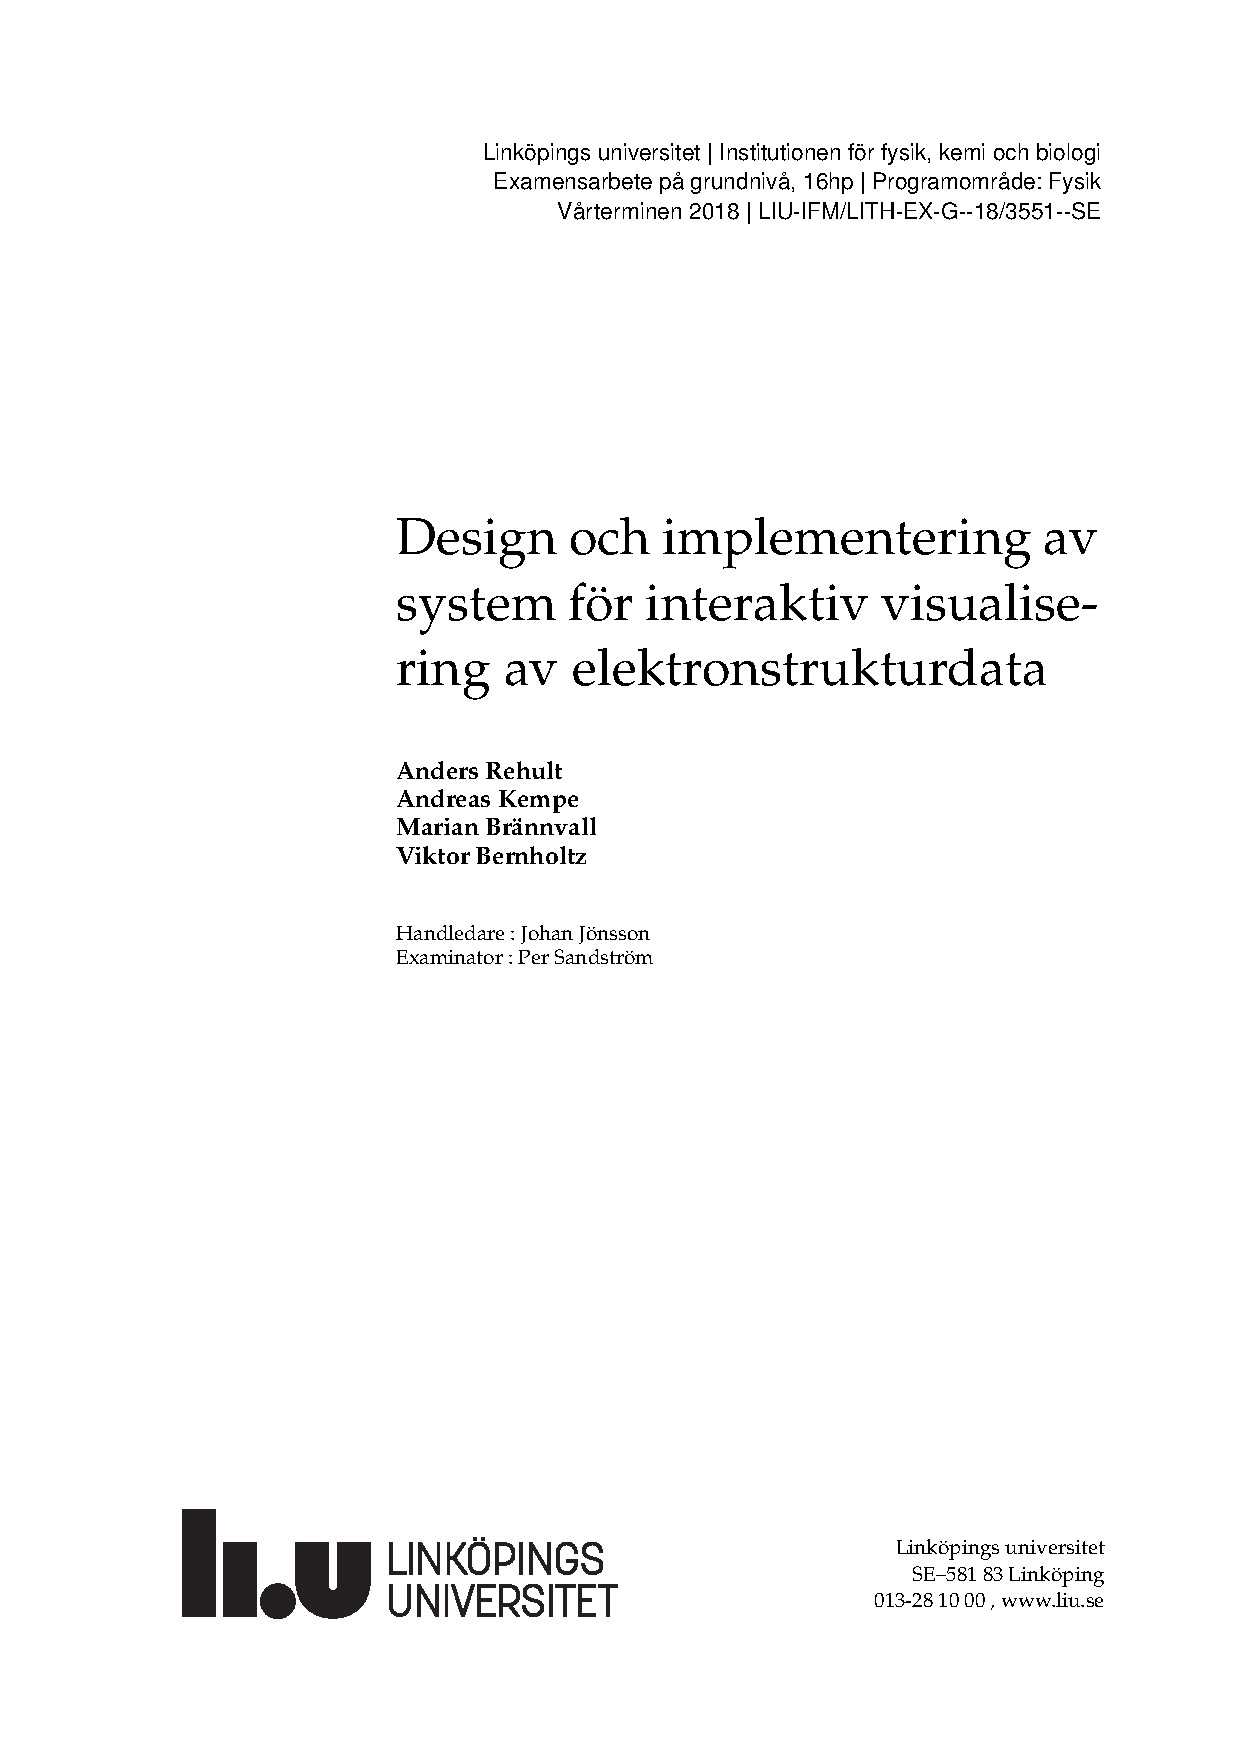
\includepdf{framsida.pdf}

\LIPStitelsida


\subsection*{Förord}
Vi vill rikta ett stort tack till vår handledare Johan Jönsson som haft stort tålamod med alla våra kursrelaterade och icke-kursrelaterade frågor under arbetets gång. Vi vill även tacka vår beställare Rickard Armiento som svarat på alla möjliga frågor och varit behjälplig under projektet.
\newpage


\begin{abstract}
Att kunna göra olika typer av visualiseringar baserat på elektronstrukturberäkningar är viktigt, bland annat för att kunna presentera resultat från forskning inom materialfysik på ett enklare sätt. Detta dokument är en slutrapport  för kandidatprojektet i visualisering av elektronstrukturer. slutrapporten beskriver bland annat projektets problemformulering och resultat, dessutom finns en beskrivning av genomförandet av projektet samt en teknisk beskrivning av det visualiseringsverktyg som tagits fram.
\newpage
\end{abstract}

\begin{LIPSprojektidentitet}
  \LIPSgruppmedlem{Anders Rehult}{Projektledare (PL)}{076-3161206}{andre449@student.liu.se}
  \LIPSgruppmedlem{\LIPSdokumentansvarig}{Dokumentansvarig (DOK)}{070-7280044}{marbr639@student.liu.se}
  \LIPSgruppmedlem{Andreas Kempe}{Sekreterare (SE)}{073-9796689}{andke133@student.liu.se}
  \LIPSgruppmedlem{Viktor Bernholtz}{Viktor Bernholtz (VB)}{073-0386030}{vikbe253@student.liu.se}
\end{LIPSprojektidentitet}

\tableofcontents{}
\newpage

\addcontentsline{toc}{section}{Dokumenthistorik}
\begin{LIPSdokumenthistorik}
  \LIPSversionsinfo{0.1}{2018-05-14}{Första utkast.}{Projektgruppen}{PL}
  \LIPSversionsinfo{0.2}{2018-05-22}{Andra utkast.}{Projektgruppen}{VB}
   \LIPSversionsinfo{0.3}{2018-05-25}{En del korrigeringar efter återkoppling från beställare.}{Projektgruppen}{}
\end{LIPSdokumenthistorik}
\newpage
\pagenumbering{arabic}

\section{Inledning}
\label{ch:inledning}
Detta dokument är en slutrapport för kandidatprojektet i visualisering av elektronstrukturer. Visualisering av elektronstrukturer är ett av projekten i kursen TFYA75 vid
Linköpings universitet. 

Inom materialfysik är elektronstrukturberäkningar viktiga teoretiska verktyg. Detta för att få en så bra förståelse som möjligt av hur olika material är uppbyggda, bland annat vad gäller kristallers egenskaper sedda ur ett kvantmekaniskt perspektiv. Det kan exempelvis handla om att man vill ta reda på olika materials egenskaper vad gäller värmeledningsförmåga, strömledningsförmåga, etc.

För att öka förståelsen samt för att enklare kunna presentera resultat från forskning inom området underlättar det att kunna göra olika typer av visualiseringar baserat på elektronstrukturberäkningar.

I många av de system som används för att utföra dessa beräkningar, exempelvis programmet VASP som utför elektronstruktur-och-molekylärdynamikberäkningar, ges ingen eller begränsad möjlighet till detta. Vidare finns begränsningar i de system som finns tillgängliga idag vad gäller effektivetet, stadardisering och tillgång till visualiseringsfunktioner.

Projektgruppen har vidareutvecklat och utökat det system som togs fram av 2017 års projektgrupp. Utöver det konkreta målet med utvecklingen av mjukvara för visualisering ska även projektet ge projektmedlemmarna erfarenhet av att arbeta i projekt och utöka deras förmåga till analytiskt och fysikaliskt tänkande för att ge värdefull erfarenhet inför arbetslivet.

Kappan ger en översikt över hela projektet och består av följande delar:

\begin{itemize}
	\item \textbf{Problemformulering}, avsnitt \ref{ch:problemformulering}, och \textbf{Kunskapsbas}, avsnitt \ref{ch:kunskapsbas}, beskriver själva förarbetet i projektet.
	
	\item \textbf{Fördjupningsarbeten}, se avsnitt \ref{ch:fördjupningsarbeten}, beskriver kortfattat de fördjupningsområden som projektgruppen behandlat.
	
	\item \textbf{Fasplan}, avsnitt \ref{ch:fasplan}, beskriver överskådligt hur projektet har genomförts.

	\item \textbf{Teknisk beskrivning}, avsnitt \ref{ch:teknisk-beskrivning}, beskriver överskådligt hur systemet är uppbyggt.
	
	\item \textbf{Resultat}, avsnitt \ref{ch:resultat}, och \textbf{Slutsats}, avsnitt \ref{ch:slutsats}, beskriver vilka krav som är uppfyllda och hur det slutgiltiga resultatet blev samt sammanfattar projektet i sin helhet.
\end{itemize}

\subsection{Parter}
Rickard Armiento har beställt systemet som är beskrivet i slutrapporten. Medlemmarna i projektgruppen, som är listade under rubriken projektidentitet ovan, är mottagare av denna beställning och har haft i uppgift att implementera systemet. Projektgruppens handledare är Johan Jönsson.


\subsection{Användning}
Denna produkt kommer användas vid Linköpings universitet för att analysera data från elektronstrukturberäkningar.

\subsection{Begränsningar}
I projektet har visualiseringsverktyget Inviwo och
programmeringspråken Python och C++ användts. Det har inte utretts huruvida andra verktyg hade varit lämpligare.

\subsection{Definitioner}

\textbf{C++} är ett programmeringsspråk.
\cite{C++}
\newline
I Inviwo används C++ för att skriva programkod till
processorer.

\textbf{Fermi-yta} är, för elektroners k-punkter i reciproka rymden, isoytan där elektronernas energi är lika med Fermi-energin.
\cite{Fermi-yta}

\textbf{HDF5} är ett filformat som kan hantera stora mängder data.
\cite{hdf5}

\textbf{Inviwo} (Interactive Visualization Workshop) är programvara
för visualisering som tillhandahåller en nätverksredigerare för
designen av dataflödesnätverk. Noderna i dessa dataflödesnätverk
kallas processorer. Indata till nätverken behandlas i dessa
processorer och utdata genereras.
\cite{Inviwo}

\textbf{Python} är ett programmeringsspråk \cite{Python}. I Inviwo används Python för att knyta samman processorer.


\section{Problemformulering}
\label{ch:problemformulering}

I projektdirektivet, se appendix \ref{appendix:projektdirektiv}, ges en översiktlig bild av de krav som kan komma att ställas på systemet. Utifrån projektdirektivet har projektgruppen skapat en kravspecifikation, se appendix \ref{appendix:kravspecifikation}, med de krav som ställs på systemet och även de generella krav som ställs på projektet och dokumentationen.

Systemet ska vara ett verktyg för att visualisera olika egenskaper från elektonstrukturberäkningar och själva visualiseringen ska ske i programvaran Inviwo \cite{Inviwo}.
Systemet ska vara uppbyggt av två huvudsakliga delsystem: ett som hanterar konvertering av data och ett annat som visualiserar den konverterade datan, se figur \ref{fig:grov-skiss}. Vilken data som visualiseras ska kunna väljas av användaren. Systemet ska vara en vidareutveckling av det system som togs fram av 2017 års projektgrupp. Projektgruppen ska utöka och uppdatera befintlig kod för att uppfylla de krav som ställts i kravspecifikationen.

\begin{figure}[H]
	\centering
	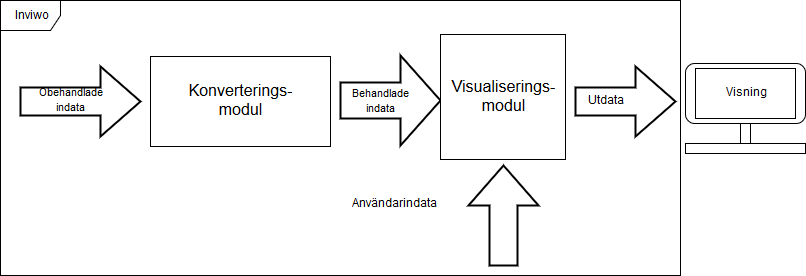
\includegraphics[scale=0.55]{grov-skiss.png}
	\caption{Grov design av systemet}
	\label{fig:grov-skiss}
\end{figure}



\section{Kunskapsbas}
\label{ch:kunskapsbas}
Projektgruppen har efter att ha tagit del av projektdirektivet, se appendix \ref{appendix:projektdirektiv},
skrivit en kravspecifikation, se appendix \ref{appendix:kravspecifikation}. Därefter skrevs en projektplan, se appendix \ref{appendix:projektplan}, tidplan, se appendix \ref{appendix:tidplan} och en  systemskiss, se appendix \ref{appendix:systemskiss}, enligt LIPS-modellen \cite{LIPS}. 
Dessa dokument har sedan fungerat som en utgångspunkt för projektets utforming. Utöver dessa har en designspecifikation skrivits, se appendix \ref{appendix:designspecifikation}, som är en fördjupning i systemskissen och ger en mer detaljerad beskrivning av systemet.

Projektgruppen har skrivit två fördjupningsarbeten, se appendix \ref{appendix:fermi-ytor} och \ref{appendix:visualisering}, knutna till projektarbetet.

Projektgruppen har tagit del av ett antal föreläsningar om dokumentationen i projektet. Utöver dessa har även föreläsningar i Inviwo och Python hållts samt laborationer i beräkningsfysik och Python-programmering. 

\section{Fasplan}
\label{ch:fasplan}
Projektet drivs enligt LIPS-modellen, som är en modell med regler, instruktioner och mallar för att bedriva projekt. Projektet delas upp i tre faser - före, under, och efter.

\subsection{Före-fas}
Före-fasen är ämnad att undersöka om projektet bör genomföras och, om så är fallet, definiera och konkretisera projektets mål samt organisera arbetet som krävs för att uppnå dessa. Under före-fasen skrivs bland annat ett projektdirektiv, se appendix \ref{appendix:projektdirektiv}, en kravspecifikation, se appendix \ref{appendix:kravspecifikation}, en systemskiss, se appendix \ref{appendix:systemskiss}, och en projektplan, se appendix \ref{appendix:projektplan}. Projektdirektivet skrevs innan projektgruppen skapades och gavs till projektgruppen vid projektets start.
Projektgruppen har under före-fasen skrivit ett gruppkontrakt, se appendix \ref{appendix:Gruppkontrakt}, en kravspecifikation, en systemskiss samt en projektplan.

\subsection{Under-fas}
Under  under-fasen  utförs  det  arbete  som  leder  till  att  projektets  krav  uppfylls.  Projektgrup-
pen skriver en designspecifikation, se appendix \ref{appendix:designspecifikation},
som beskriver hur systemet ska konstrueras mer detaljerat än
systemskissen. Projektgruppen arbetar sedan med att, utgående från denna designspecifikation, konstruera och testa systemet. En teknisk dokumentation, se appendix \ref{appendix:teknisk-dokumentation}, skrivs parallellt med systemets konstruktion för att reflektera den faktiska implementationen av idéerna beskrivna i designspecifikationen. 

Projektgruppen har också skrivit en naturvetenskaplig undersökning och två fördjupningsarbeten knutna till projektet. Det ena fördjupningsarbetet, se appendix \ref{appendix:fermi-ytor}, behandlar Fermi-ytor som är ett av fördjupningsområdena i projektet och som ska visualiseras. Det andra fördjupningsarbetet, se appendix \ref{appendix:visualisering}, behandlar visualisering som är en mer generell del av projektet. Den naturvetenskapliga undersökningen är en analys av visualiseringar skapade med ENVISIoN, se appendix \ref{appendix:naturvetenskaplig}.

\subsection{Efter-fas}
Under efter-fasen överförs projektresultatet till beställaren och projektet avslutas. Projektgruppen skriver en slutrapport som bifogas vid slutleveransen av produkten och även en användarmanual, se appendix \ref{appendix:anvandarmanual}. Vid slutleveransen ska
även en demonstration hållas som visar att produkten uppfyller kraven ställda på den. Efter produkten levererats skriver projektgruppen en efterstudie.

\section{Fördjupningsarbeten}
\label{ch:fördjupningsarbeten}
Nedan beskrivs kortfattat de fördjupningsarbeten som gjorts under projektet. Dessa finns i sin helhet i appendix \ref{appendix:fermi-ytor} och \ref{appendix:visualisering}. 
\subsection{Fermi-ytor}
Syftet med fördjupningsarbetet om Fermi-ytor var att besvara följande frågor: Vad är Fermi-ytor och hur kan dessa beräknas numeriskt? Detta var av intresse för projektet eftersom en del av det bestod av att visualisera Fermi-ytor. Arbetet beskriver kortfattat begrepp inom fasta tillståndets fysik som är av betydelse för att förstå vad Fermi-ytor är, för att sedan gå in på hur dessa kan beräknas numeriskt.

\subsection{Visualisering av volymdata}
I fördjupningsarbetet om visualisering av volymdata tittades det närmare på ett par av de metoder mjukvaran Inviwo använder sig av. Detta för att kunna göra en jämförelse av både prestanda och resultat mellan de två metoderna.
\section{Teknisk beskrivning}
\label{ch:teknisk-beskrivning}

Systemet hanterar indata från VASP. Datan kommer från elektronstrukturberäkningar och konverteras till HDF5-format för att därefter visualiseras. Användaren kan välja vad som ska visualiseras, kontrollera renderingens utseende och ställa in egenskaper såsom färg, transparens, och rotation. Systemet har delats in i delsystem och dessa har utvecklats och testats enskilt i den mån det inte funnits beroenden till andra delsystem.

I avsnitt \ref{ch:datakonvertering} och \ref{ch:visualisering} nedan ges en övergripande inblick i det två huvudsakliga delsystemen och deras delsystem. För en mer detaljerad teknisk beskriving av systemet se den tekniska dokumentationen, se appendix \ref{appendix:teknisk-dokumentation}.

\subsection{Datakonvertering}
\label{ch:datakonvertering}
Detta avsnitt behandlar delsystemet datakonvertering, figur \ref{fig:konverteringdetalj} ger en grov översikt av delsystemet. Obehandlad data skickas in där obehandlad data är i form av textfiler med data från beräkningar gjorda i VASP. Indata behandlas sedan i konverteringsmodulen. Från konverteringsmodulen kommer behandlad data i HDF5-format.

\begin{figure}[H]
	\centering
	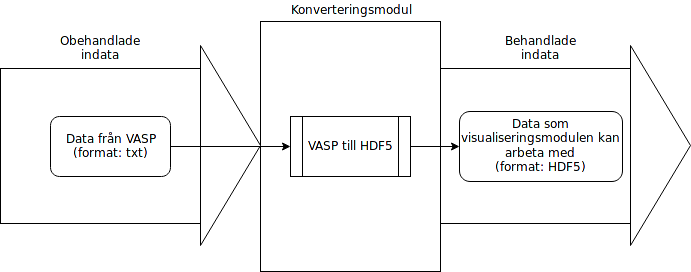
\includegraphics[scale=0.55]{konverteringdetalj.png}
	\caption{Grov design av konverteringsmodulen}
	\label{fig:konverteringdetalj}
\end{figure}

\subsubsection{HDF5}
Systemet kan hantera olika utdatafiler från VASP. Detta görs genom att datan konverteras till HDF5-format.
HDF5 är ett filformat som är designat för att hantera stora mängder data på ett flexibelt sätt \cite{hdf5}.
HDF5 har flera olika datatyper och ett HDF5-objekt som antingen är lagrat på disk eller hålls i minnet är uppdelat i två huvudsakliga underobjekt, nämligen grupper och dataset.


Alla HDF5-objekt har en rotgrupp som äger alla andra objekt i datastrukturen. Denna grupp innehåller i sin tur all övrig data i form av andra grupper, länkar till andra grupper, eller dataset.
Dataset innehåller rådata av något slag. Rådata kan i sammanhanget vara bilder, utdata från beräkningar, programdata, etc.
I designspecifikationen, se appendix \ref{appendix:designspecifikation}, ges en mer detaljerad beskriving av HDF5.

\subsubsection{VASP}
Från beräkningsprogrammet VASP fås en rad olika utdatafiler. Dessa listas och beskrivs i designspecifikationen, se appendix \ref{appendix:designspecifikation}. Ur dessa utdatafiler läses saker som atompositionsdata, gittervektorer, elektrontäthetsdata, tillståndstäthetsdata, Fermi-energi, och så vidare för att kunna visualisera kristallstrukturer, elektrontäthet, elektronlokaliseringsfunktionen (ELF), tillståndstäthet, och Fermi-ytor. I designspecifikationen beskrivs närmare vad som läses från vilka utdatafiler. 

\subsection{Visualisering}
\label{ch:visualisering}
Figur \ref{fig:visualisering} visar hur delsystemet för visualisering är uppbyggt. Behandlad data samt användarindata skickas in. Användarindata består av val av färg, val av egenskap som ska ritas ut, val av transparens etc. Dessa behandlas i visualiseringsmodulen som skapar en bild utifrån dem. Den utritade bilden skickas sedan ut från modulen. Detta är en allmän beskrivning av visualiseringen - mittenrektangeln i figur \ref{fig:visualisering} är för de olika egenskaperna som visualiseras uppbyggd på olika sätt med olika processorer.
\label{visualisering}
\begin{figure}[H]
	\centering
	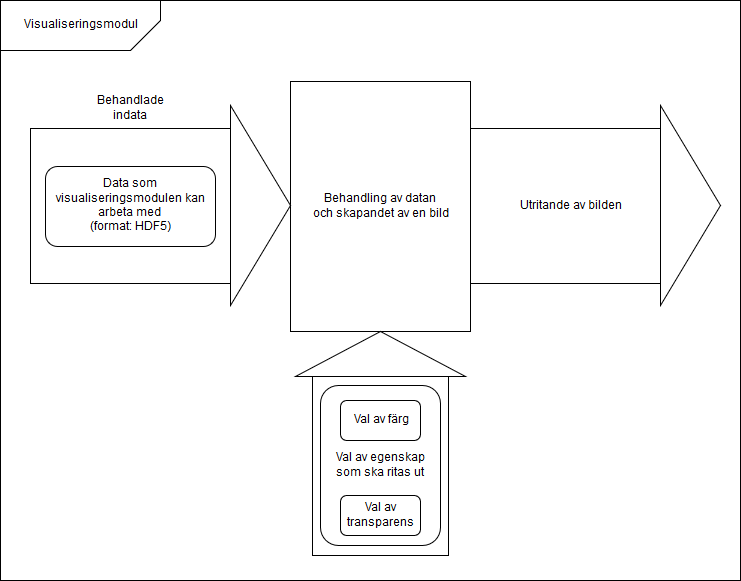
\includegraphics[scale=0.45]{Visualisering.png}
	\caption{Grov design av delsystemet för visualisering}
	\label{fig:visualisering}
\end{figure}
\subsubsection{Utritning}
Delsystemet ritar ut bilder utefter den behandlade datan. Utritningen ger en visualisering av den egenskap som modulen behandlar och kan till exempel vara en volymrendering eller en 2D-graf, beroende på vilket som är mest lättolkat. 

Utritningen görs via Inviwos inbyggda funktionalitet för att rendera via OpenGL som är ett API för att hantera grafik. 


\subsubsection{Användarindata}
Användaren kan ändra inställningar som kontrollerar utseendet på visualiseringarna.
Denna indata matas in i Inviwos användargränssnitt via inställningsrutan för en processor. Figur \ref{fig:interface} visar vad användaren ser när ELF-data för diamant visualiseras. Längst till vänster i figuren ses ett fönster med Properties, i detta fall för processorn ELF raycasting som kan hittas i nätverket längst till höger i figuren. I mitten av figuren ligger den utritade bilden. Bilden kan roteras genom att klicka och dra i den. I fönstret Properties finns en egenskap vid namn Transfer function, med hjälp av vilken användaren kan ändra transparens/opacitet samt färg, se figur \ref{fig:transferfunction}.

\begin{figure}[H]
	\centering
	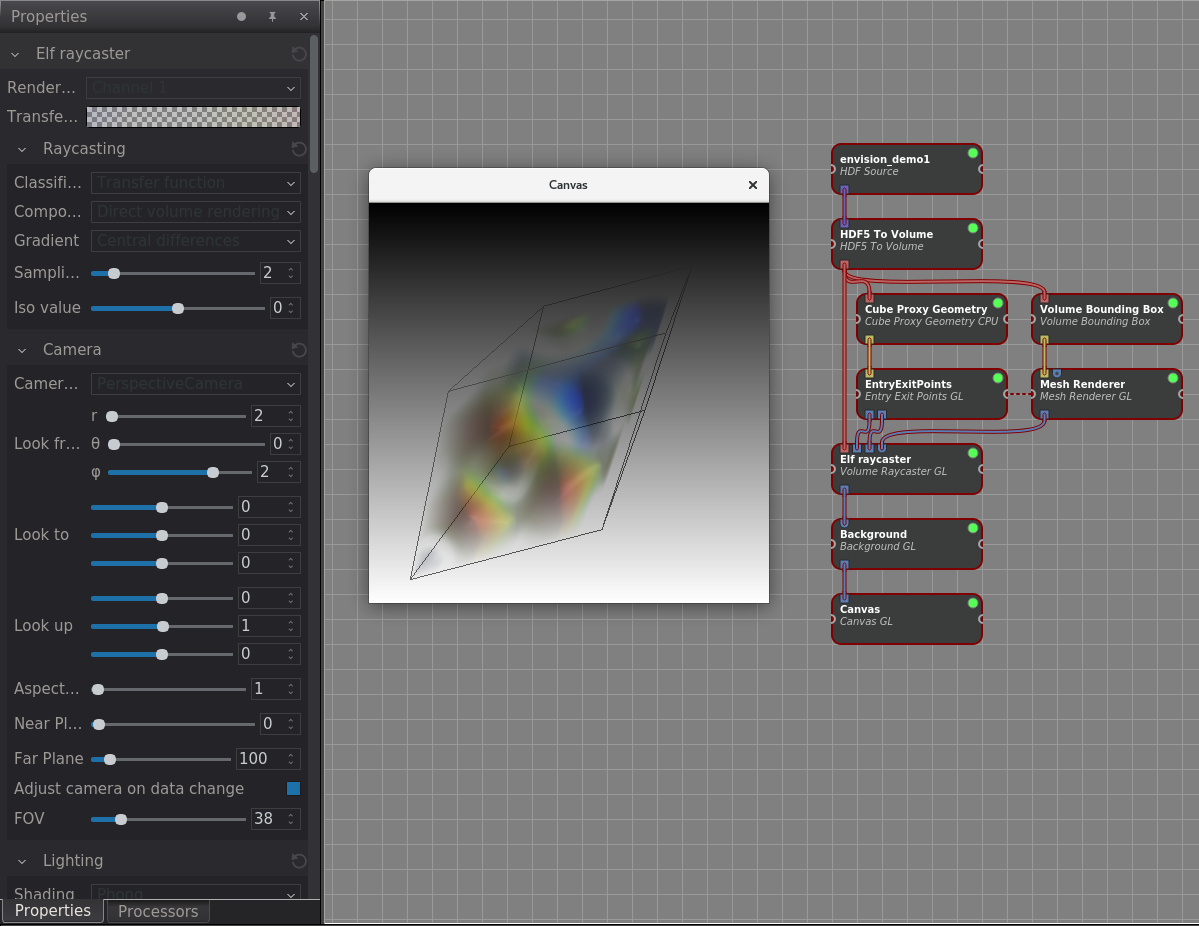
\includegraphics[scale=0.3]{inviwo_interface_elf.png}
	\caption{Bild av vad användaren ser när ELF visualiseras, i detta fall för diamant.}
	\label{fig:interface}
\end{figure}

\begin{figure}[H]
	\centering
	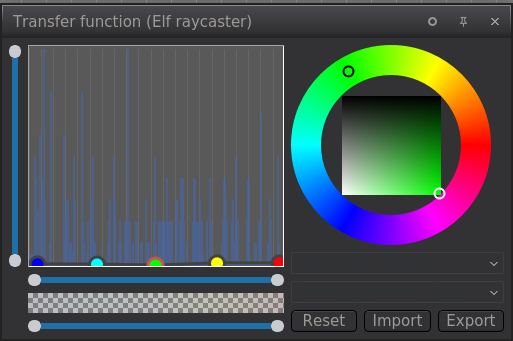
\includegraphics[scale=0.55]{transferfunction_elf.png}
	\caption{Transfer function property där transparens och färg kan ställlas in.}
	\label{fig:transferfunction}
\end{figure}

Visualiseringsfunktionaliteten läggas till i form av processorer som via Inviwo tillhandahåller inställningsmöjligheter på det sätt som beskrivits i designspecifikationen, se appendix \ref{appendix:designspecifikation}. Således blir inte användarinställningar ett eget separat delsystem, utan kommer att bakas in i visualiseringssystemen. Detta görs genom att processorerna är skrivna att exponera de inställningar som användaren är menad att
justera. Inviwo kommer då automatiskt lägga till inställningarna i rutan.

\subsubsection{Interaktivitet}
Användaren kan modifiera visualiseringen genom att reglera ett intervall av värden för
någon egenskap där full transparens fås för alla värden inom intervallet, rotera 3D-bilder etc.
Ny användarindata, som skickas in efter att den första bilden har ritats upp, skickas tillbaka till
visualiseringsmodulen för att utföra en ny rendering. 

\subsubsection{Kristallstruktur}
Kristallstruktur visualiseras som atompositioner i enhetscellen. Sfärer som representerar atomer  kan  ritas  ut  genom  volymsrendering. % figur och exempel?
I designspecifikationen, se appendix \ref{appendix:designspecifikation}, finns en mer detaljerad beskrivning av
hur detta byggs upp. I kap. \ref{ch:resultat} i figur \ref{fig:visualisering_TiPO4} ses ett exempel på denna typ av visualisering.


\subsubsection{Elektrontäthet}
Elektrontäthet visualiseras genom volymsrendering. Det är sannolikheten för att hitta elektroner på olika positioner som visualiseras.
I designspecifikationen, se appendix \ref{appendix:designspecifikation}, finns en mer detaljerad beskrivning av elektrontäthet. I kap. \ref{ch:resultat} i figur \ref{fig:visualisering_NaCl_slice} och figur \ref{fig:visualisering_NaCl_iso} ses två exempel på denna typ av visualisering.

\subsubsection{ELF}
Data för elektronlokaliseringsfunktionen (electron localization function, ELF) visualiseras på liknande sätt som elektrontäthet eftersom även det är volymdata som ska visualiseras. Hur ELF visualiseras beskrivs mer detaljerat i den tekniska dokumentationen, se appendix \ref{appendix:teknisk-dokumentation}. I kap. \ref{ch:resultat} i figur \ref{fig:visualisering_diamant_elf} ses ett exempel på denna typ av visualisering.

\subsubsection{Tillståndstäthet}
Tillståndstäthet visualiseras med en 2D-graf med energin på x-axeln och tillståndstätheten på y-axeln. 
I designspecifikationen, se appendix \ref{appendix:designspecifikation}, finns en mer detaljerad besrivning av tillståndstäthet. I kap. \ref{ch:resultat} i figur \ref{fig:visualisering_total_DOS_Cu} ses ett exempel på denna typ av visualisering.

\subsection{Sammanlänkning av olika visualiseringar}
Det finns även möjlighet att visualisera kristallstrukturer tillsammans med elektrontähet, ELF eller tillståndstäthet. I kap. \ref{ch:resultat} i figur \ref{fig:visualisering_sammanlankning} ses ett exempel på denna typ av visualisering.

\section{Resultat}
\label{ch:resultat}
Projektet bestod av att skapa ett visualiseringsverktyg i Inviwo som ska kunna visualisera resultat från elektronstrukturberäkningar. Det framtagna visualiseringsverktyget ska uppfylla kraven från kravspecifikationen, nedan beskrivs några av kraven som ställts på systemet samt huruvida dessa är uppfyllda.

\subsection{Krav på systemet}
Tabell \ref{table:kravlista generella systemet} är en kravlista med några utvalda krav på det generella systemet. För samtliga krav se kravspecifikationen i appendix \ref{appendix:kravspecifikation}. Krav fem är ett krav på egenskaper som ska kunna visualiseras. Projektgruppen valde att implementera visualisering av Fermi-ytor och Total DOS, men även visualisering av ELF har implementerats. 2017 års projektgrupp i visualisering implementerade ur listan i krav fem visualisering av total DOS, visualisering av ELF-data, och visualisering av bandstruktur. Detta års arbete bestod i att uppdatera majoriteten av den skrivna koden till att vara kompatibel med version 0.9.9 av Inviwo. Krav 45 är ett ska-krav som säger att koden ska fungera för version 0.9.9 eller senare versioner av Inviwo. Att uppdatera befintlig kod visade sig bli en stor del av arbetet eftersom tidigare versioner av Inviwo skilde sig mycket från version 0.9.9 då Inviwo uppdaterat sitt python stöd i grunden.
 

\begin{table}[H]
\caption{Reducerad kravlista för det generella systemet.}
\begin{center}
\begin{tabular}{ |p{10mm}|p{20mm}|p{70mm}|p{15mm}|p{15mm}|}
\hline
 \textbf{Krav} & \textbf{Förändring} & \textbf{Beskrivning} & \textbf{Prioritet} & \textbf{Uppfyllt}  \\ 
\hline
 5 & Omförhand\-lat 2018-05-21 & Projektgruppen ska utöka alternativt implementera visualisering av minst en av nedanstående  egenskaper, samt uppdatera minst en redan existerande implementation av någon av de nedanstående egenskaperna:
  \begin{itemize}
  \item Elastiska konstanter
  \item Fermi-ytor
  \item ELF (Electron Localization Function)
  \item Krafter på atomer
  \item Bandstruktur
  \item Total DOS (Density Of States)
  \item Parkorrelationsfunktionen
  \item Illustration av partiell elektrondensitet
  \end{itemize} & Ska & Ja \\
\hline
7 & Original & Tillhandahållna python-moduler ska kunna anropas med enkla funktionsanrop. & Ska & Ja \\
\hline
13 & Original & Användaren ska kunna välja vilken typ av visualisering som ska visas. & Ska & Ja \\
\hline
14 & Original & Användaren ska kunna länka samman olika python-moduler. & Ska & Ja \\
\hline
15 & Original & Systemet ska implementeras i Inviwo. & Ska & Ja \\
\hline
18 & Original & Tillhandahållna python-moduler ska inte fortskrida som vanligt vid indata av fel typ. & Ska & Ja \\
\hline
19 & Original & Tillhandahållna python-moduler ska vid felaktig indata varna användaren. & Ska & Ja \\
\hline
45 & Original & Koden ska fungera för Inviwo 0.9.9 eller någon efterkommande version. & Ska & Ja \\
\hline

\end{tabular}
\label{table:kravlista generella systemet}
\end{center}
\end{table}

I krav 5 valde projektgruppen att utöka implementeringen för Total DOS som kan ses i figur \ref{fig:visualisering_total_DOS_Cu} som visar en 2D-graf som ritar upp total tillståndstäthet för koppar, Cu.
\begin{figure}[H]
	\centering
	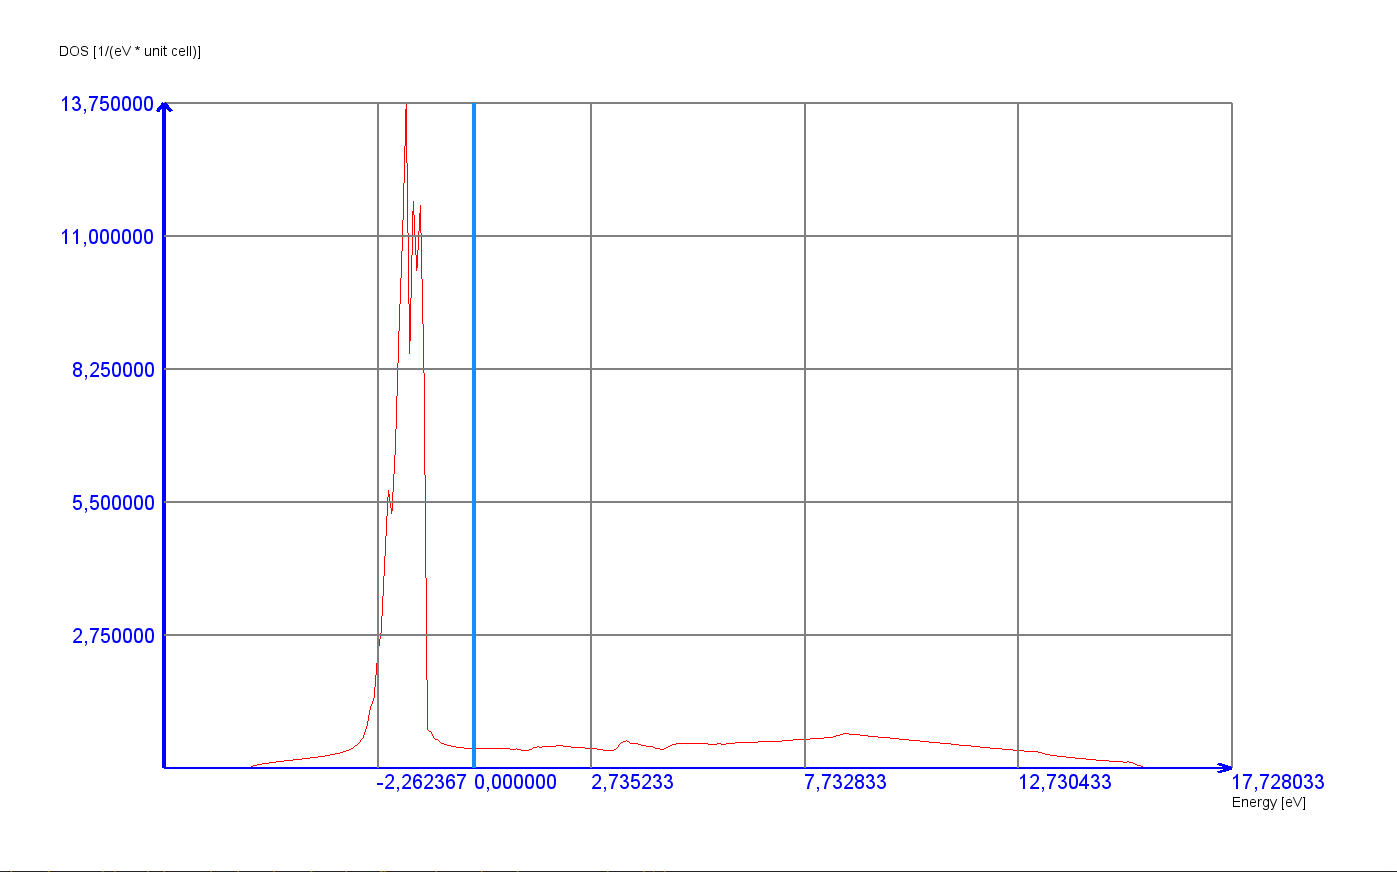
\includegraphics[scale=0.3]{Cu_1_10_total_DOS_visualisering.png}
	\caption{Visualisering av total tillståndstäthet för Cu.}
	\label{fig:visualisering_total_DOS_Cu}
\end{figure}

Även befintlig kod för visualisering av ELF har uppdaterats. Figur \ref{fig:visualisering_diamant_elf} visar visualisering av ELF-data för diamant. 
\begin{figure}[H]
	\centering
	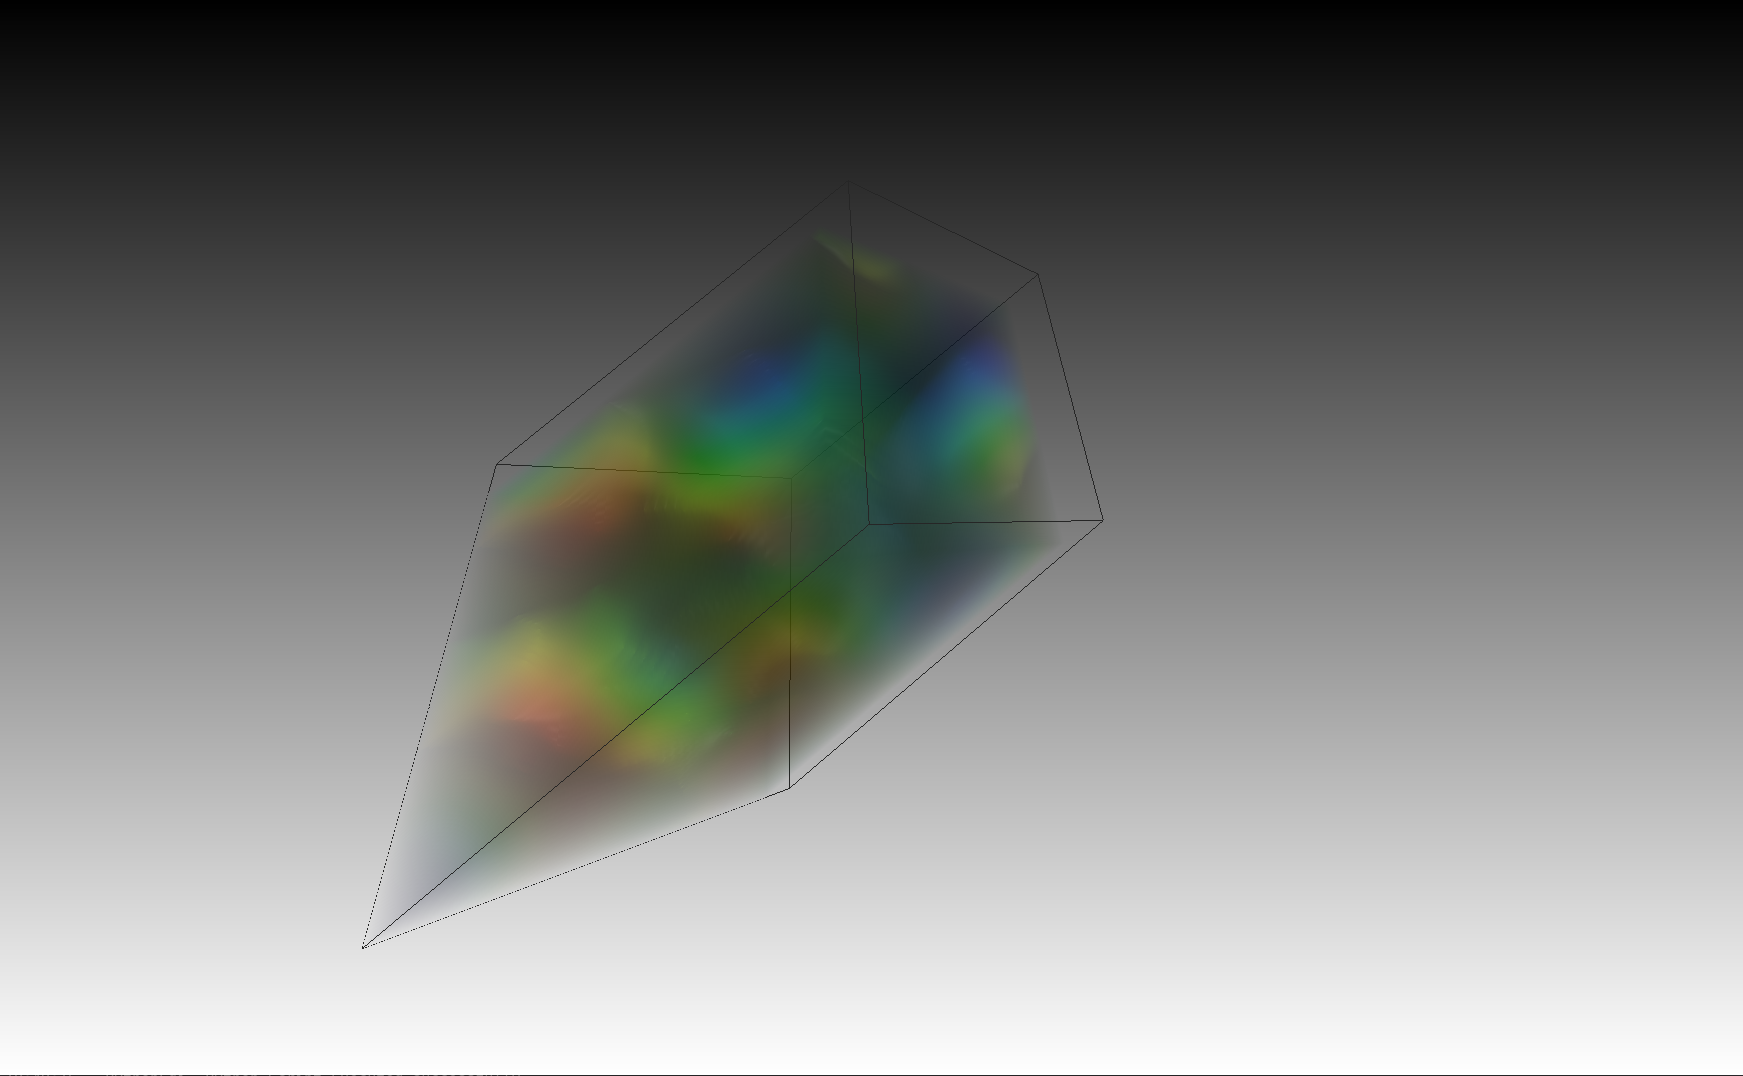
\includegraphics[scale=0.15]{Diamant_elf_visualisering.png}
	\caption{Visualisering av ELF-data för diamant.}
	\label{fig:visualisering_diamant_elf}
\end{figure}

Figur \ref{fig:visualisering_sammanlankning} visar hur visualiseringen för en sammanlänkning mellan utritande av enhetscell och utritande av ELF kan se ut, i detta fall för aluminium. Detta uppfyller alltså krav 14. Sammanlänkning kan göras mellan kristallstruktur och volymdata (laddningstäthet och ELF) eller mellan kristallstruktur och tillståndstäthet. Det senare gör det möjligt att se projicerad tillståndstäthet genom att klicka på enskilda atomer, vilket är krav 36 i tabell \ref{table:kravlista visualisering}.
\begin{figure}[H]
	\centering
	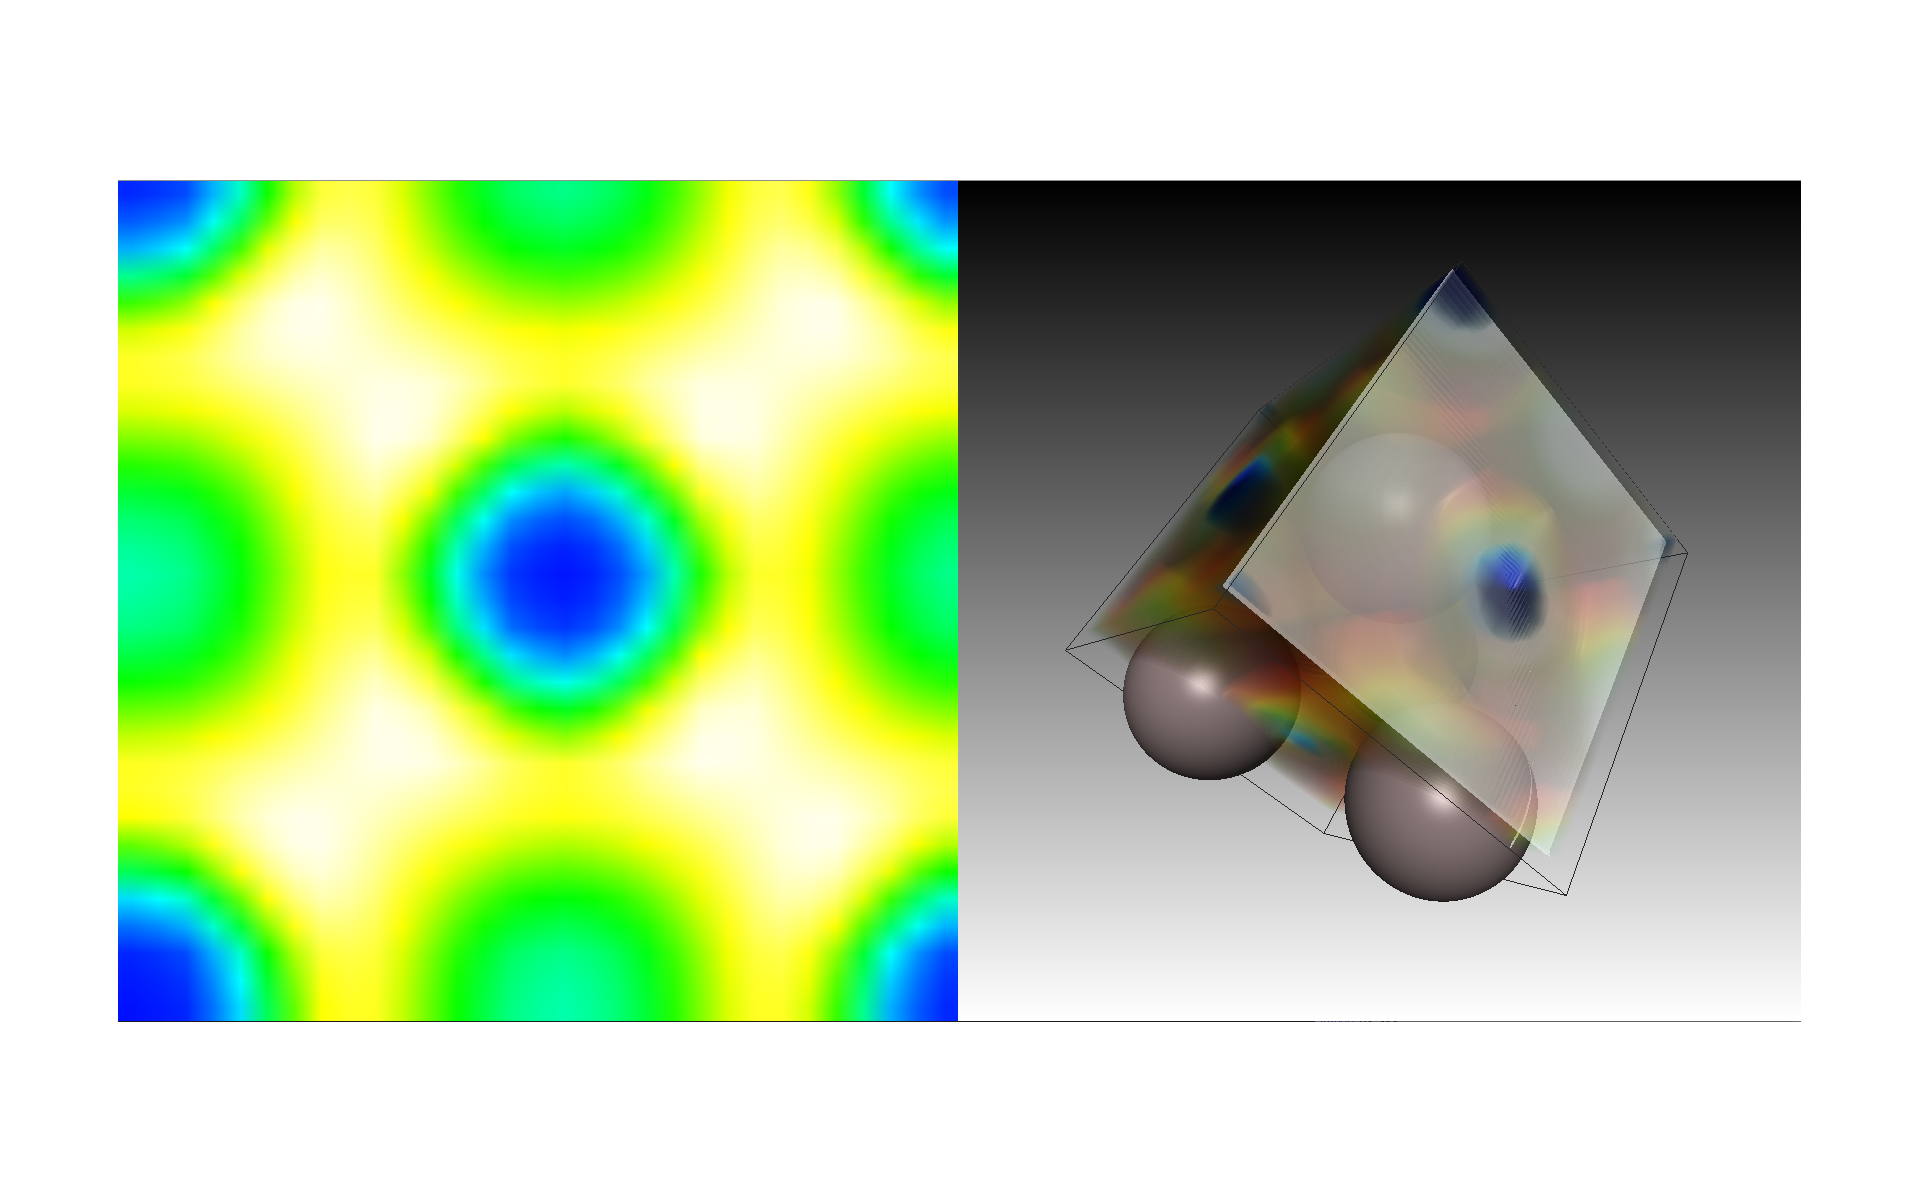
\includegraphics[scale=0.2]{sammanlankning_visualisering_Al.png}
	\caption{Data för enhetscell och ELF för aluminium visualiseras i samma bild.}
	\label{fig:visualisering_sammanlankning}
\end{figure}

I tabell \ref{table:kravlista datakonvertering} ses några av de krav som ställts på delsystemet för datakonvertering. Krav 24 och 29 är krav på vilket beräkningsprogram som systemet ska kunna läsa in resultat ifrån. Krav 25, 26 och 27 är krav på vilka data som ska kunna läsas in och krav 28 är ett krav på till vilket filformat som datan ska konverteras. 
\begin{table}[H]
\caption{Reducerad kravlista för delsystemet för datakonvertering.}
\begin{center}
\begin{tabular}{ |p{10mm}|p{20mm}|p{70mm}|p{15mm}|p{15mm}|}
\hline
 \textbf{Krav} & \textbf{Förändring} & \textbf{Beskrivning} & \textbf{Prioritet} & \textbf{Uppfyllt}  \\ 
\hline
24 & Original & Systemet ska kunna läsa in resultat från VASP. & Ska & Ja \\
\hline
25 & Original & Systemet ska kunna konvertera data från kristallstrukturberäkningar. & Ska & Ja \\
\hline
26 & Original & Systemet ska kunna konvertera data från elektronstrukturberäkningar. & Ska & Ja \\
\hline
27 & Original & Systemet ska kunna konvertera data från tillståndstäthetsberäkningar. & Ska & Ja \\
\hline
28 & Original & Systemet ska översätta input-filer i textformat till det binära filformatet HDF5. & Ska & Ja \\
\hline
29 & Original & Systemet bör kunna läsa in resultat från något annat beräkningsprogram, t.ex. Elk & Bör & Nej \\
\hline
\end{tabular}
\label{table:kravlista datakonvertering}
\end{center}
\end{table}


I tabell \ref{table:kravlista visualisering} ses några av de krav som ställts på delsystemet för visualisering. Visualisering av projicerad tillståndstäthet, kristallstruktur, och elektrontäthet implementerades av 2017 års projektgrupp, och det relaterade arbetet detta år bestod i att uppdatera koden för dessa visualiseringar till att vara kompatibla för version 0.9.9 av Inviwo. 

\begin{table}[H]
\caption{Reducerad kravlista för delsystemet för visualisering.}
\begin{center}
\begin{tabular}{ |p{10mm}|p{20mm}|p{70mm}|p{15mm}|p{15mm}|}
\hline
 \textbf{Krav} & \textbf{Förändring} & \textbf{Beskrivning} & \textbf{Prioritet} & \textbf{Uppfyllt}  \\ 
\hline
36 & Original & Systemet ska visualisera projicerad tillståndstäthet härrörande till varje separat atom i en kristalls enhetscell. & Ska & Ja \\
\hline
37 & Original & Systemet ska viusalisera kristallstruktur som atompositioner i enhetscellen. & Ska & Ja \\
\hline
38 & Original & Systemet ska kunna visualisera den elektrontäthet som resulterar från en beräkning. & Ska & Ja \\
\hline
\end{tabular}
\label{table:kravlista visualisering}
\end{center}
\end{table}

Figur \ref{fig:visualisering_TiPO4} är ett exempel på visualisering av kristallstruktur, krav 37. Här är det TiPO4 som ritas ut där de röda sfärerna är syreatomer, de grå är titanatomer, och de orangea är fosforatomer.
\begin{figure}[H]
	\centering
	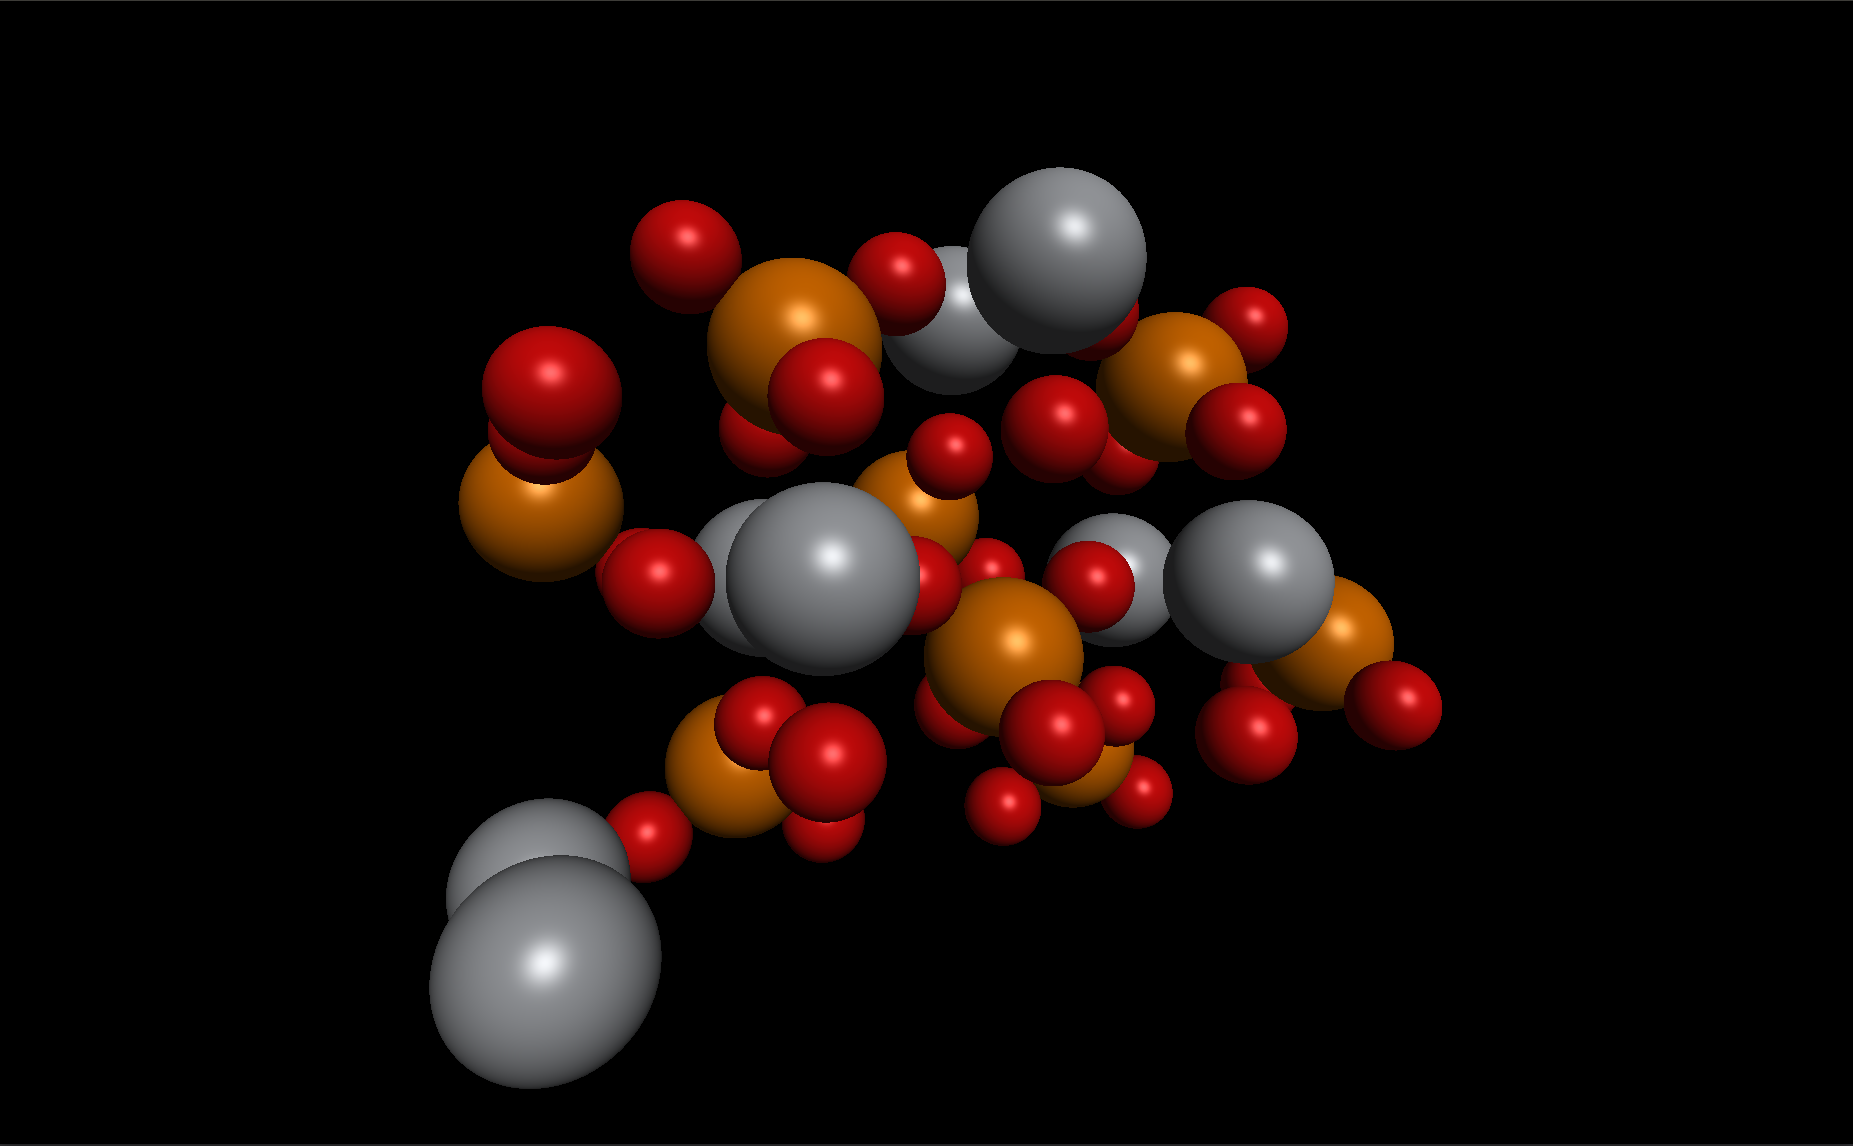
\includegraphics[scale=0.15]{TiPO4_visualisering.png}
	\caption{Visualisering av TiPO4.}
	\label{fig:visualisering_TiPO4}
\end{figure}

Figur \ref{fig:visualisering_NaCl_slice} är ett exempel på visualisering av elektrontäthet, krav 38. Här är det laddningstätheten för NaCl som ritas ut. I figur  \ref{fig:visualisering_NaCl_iso} visas även ett exempel på visualisering av laddningstäthet men i detta fall har en isoyta ritats ut för laddningstäthet lika med 0.15, även här för NaCl.

\begin{figure}[H]
	\centering
	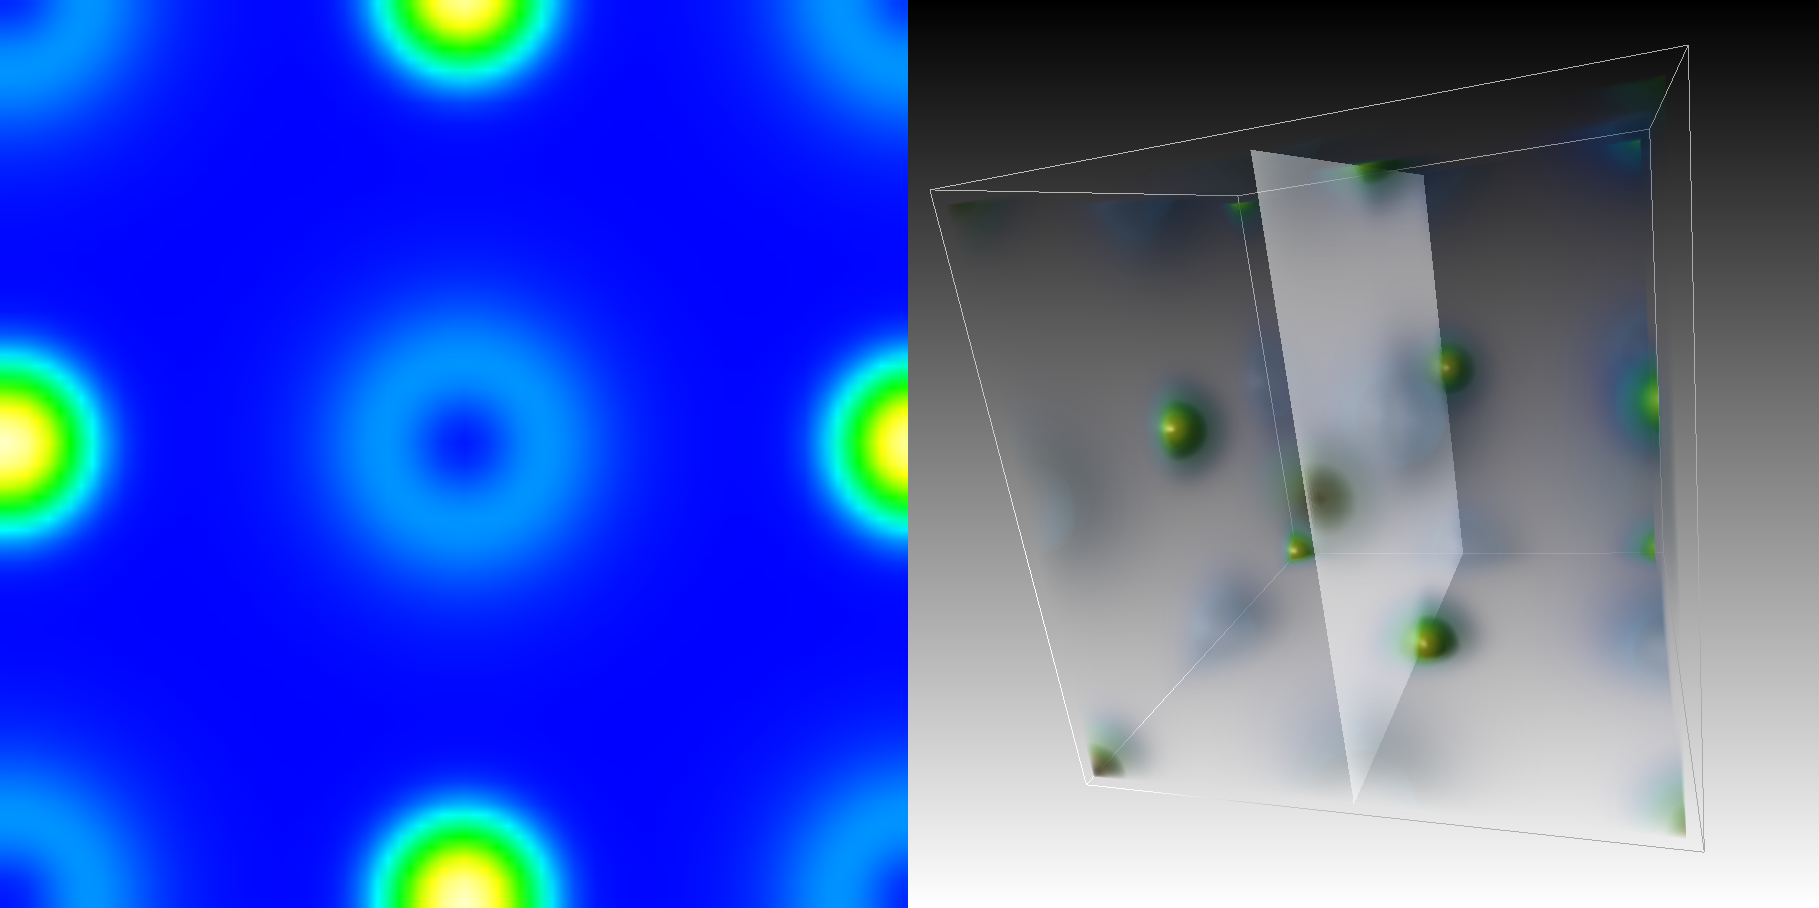
\includegraphics[scale=0.15]{NaCl_laddningstathet_slice_visualisering.png}
	\caption{Visualisering av laddningstäthet för NaCl med slice-funktion.}
	\label{fig:visualisering_NaCl_slice}
\end{figure}

\begin{figure}[H]
	\centering
	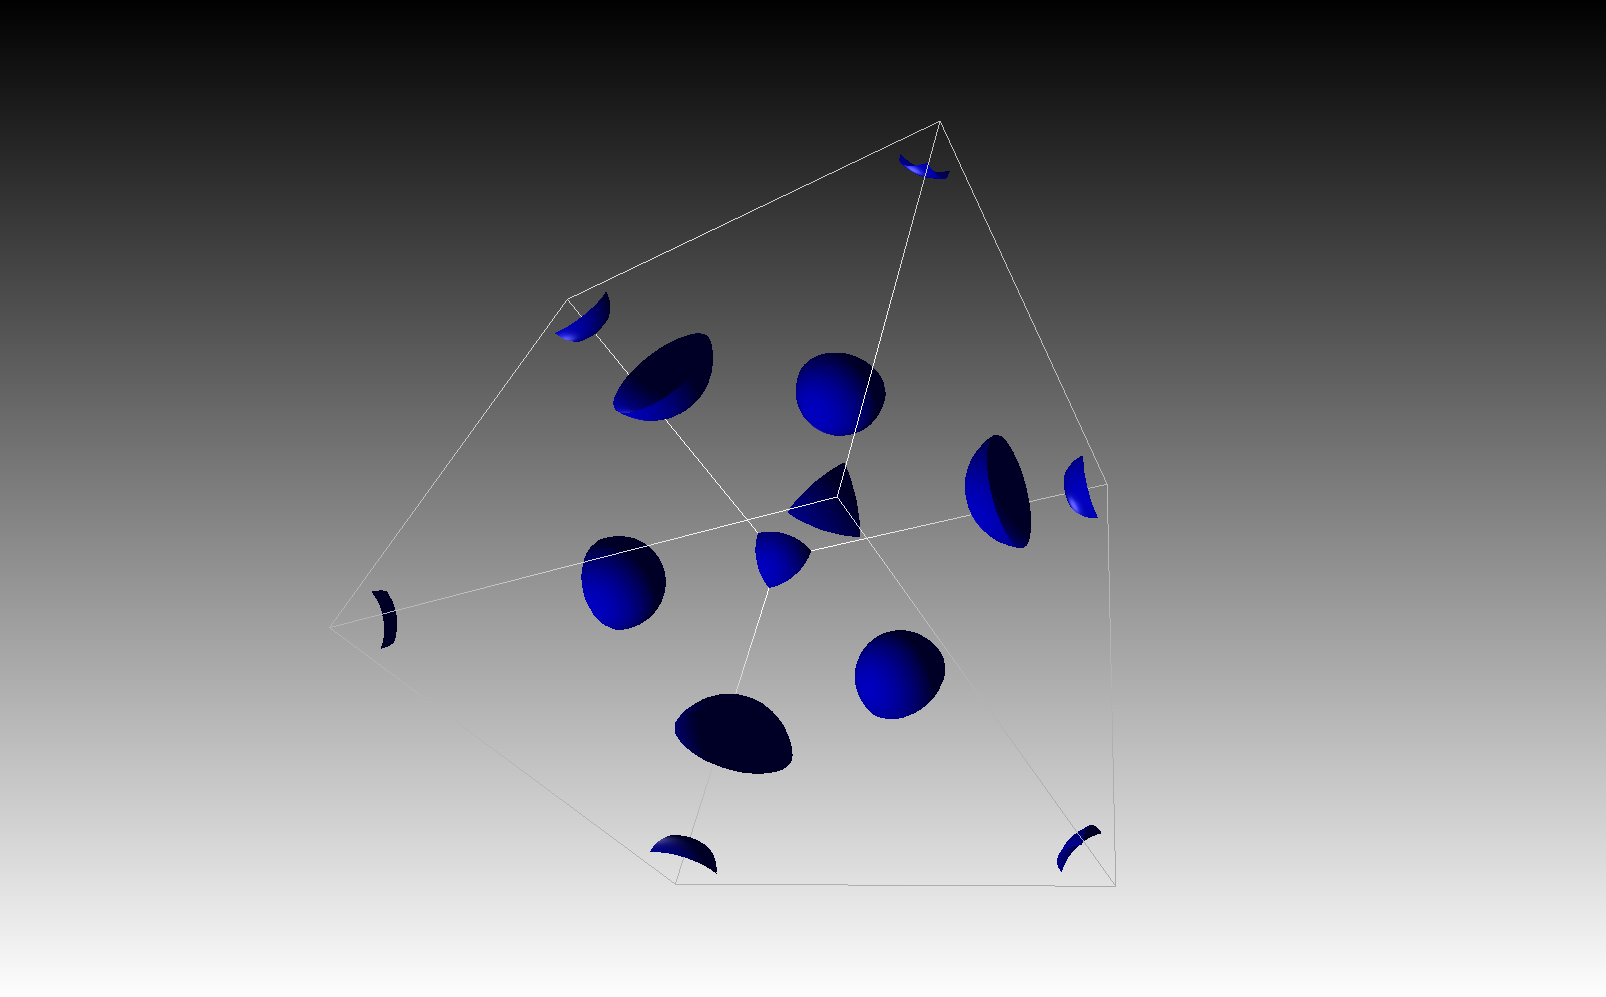
\includegraphics[scale=0.15]{NaCl_laddningstathet_iso_visualisering.png}
	\caption{Visualisering av isoyta för laddningstäthet lika med 0.15 för NaCl.}
	\label{fig:visualisering_NaCl_iso}
\end{figure}

\subsection{Användning}
För närmare beskrivning av hur verktyget används se användarmanualen i appendix \ref{appendix:anvandarmanual}. Det framtagna visualiseringsvertyget används genom att öppna programmet Inviwo och därifrån köra önskat Python-skript. Python-skript finns för samtliga typer av visualiseringar och kräver endast små ändringar i koden för att köras. Vilka ändringar som behöver göras beskrivs dels i användarmanualen men även som kommentarer i skripten.

\section{Slutsats}
\label{ch:slutsats} 
Projektarbetet har medfört ett antal lärdomar och insikter. I början av projektet skulle flera dokument skrivas som skulle vara till grund för designen av systemet som skulle implementeras samt genomförandet av projektet. Detta upplägg medförde vissa problem eftersom det krävde mycket kunskap inom främst Inviwo. Nedan beskrivs några slutsaster kring projektet inom några olika områden.

\subsection{Tekniskt}
Versionerna av Inviwo skilde sig mer än förväntat vilket gjorde att
mer tid än beräknat har gått till att uppdatera kod samt lösa problem
med Inviwo. Detta har gjort att den tekniska biten har varit väldigt
tung. Projektgruppen känner att det gärna hade fått vara mer fokus på
visualiseringsproblem och beräkningsfysik än på tekniska problem.
Planeringen av projektet utgick snarare från att eventuella problem
som skulle uppstå skulle handla om förståelse av de egenskaper som
skulle visualiseras. Problemen som uppstod med Inviwo krävde mycket
specialkunskap för att lösas vilket gjorde att en i gruppen fick lägga
mycket tid på sådant, vilket syns i tidsfördelning av nedlagd tid. 

Programmeringen har varit väldigt lärorik för flera i gruppen. Att
uppdatera 2017 års kod har, trots att det svalde mycket tid, varit
nyttigt och gett förståelse för visualiseringen. Det har även varit
lärorikt att få arbeta i ett lite större projekt, att få planera
arbetet och att lösa problem som dykt upp längs vägen. 

Under projektets gång har versionshanteringssystemet Git använts för
att versionshantera kod och typsättningssystemet LaTeX använts för att
skriva dokument, detta har varit väldigt värdefullt att sätta sig in i
och använda eftersom det med stor sannolikhet är till nytta även
utanför projektet. 
\subsection{Utförande}
I början av projektet bestod arbetet av att skriva de olika dokument som projektarbetet sedan skulle utgå ifrån. Detta var svårt eftersom det saknades mycket kunskap inom Inviwo som  var en central del i projektet. Projektgruppen känner sig nöjda med de producerade dokumenten även om t.ex. krav i kravspecifikationen i efterhand kunde ha formulerats annorlunda och varit mer tydliga, vilket var svårt att inse i början av projektet. Det hade varit bra med mer tid i början av projektet, innan skrivning av dokument påbörjades, där en slags förstudie hade kunnat göras för att sätta sig in i projektet. Detta hade kunnat ge en bättre bild av vad som behövde göras så att kravspecifikation och designspecifikation kunde skrivas mer detaljerat och korrekt. 

En i gruppen var mer kunnig i programmering än de andra. Detta var mycket värdefullt för gruppen eftersom problem som hade varit mycket komplicerade att lösa för övriga projektmedlemmar ändå kunde lösas. Dock medförde det också att tidsfördelningen av nedlagd arbetstid inte blev helt jämn inom gruppen.  

\subsection{Framtida arbete}
En idé hade varit att göra om saker från grunden istället för att uppdatera 2017 års kod. Det är dock oklart om detta verkligen hade gjort att saker gått snabbare eftersom problem med Inviwo ändå hade uppstått, men dessa hade möjligtvis kunnat kringgås på andra sätt. Arbetet hade möjligtvis kunnat parallelliseras mer men detta hade krävt mer förståelse av Inviwo från början och en bättre insikt i hur stora ändringar som behövde göras för att göra koden kompatibel med version 0.9.9 av Inviwo.  

Arbetet har känts effektivt, de nedlagda timmarna har använts bra. 



\newpage
\addcontentsline{toc}{section}{Referenser}
\printbibliography{}

\begin{appendices}
	
\newpage


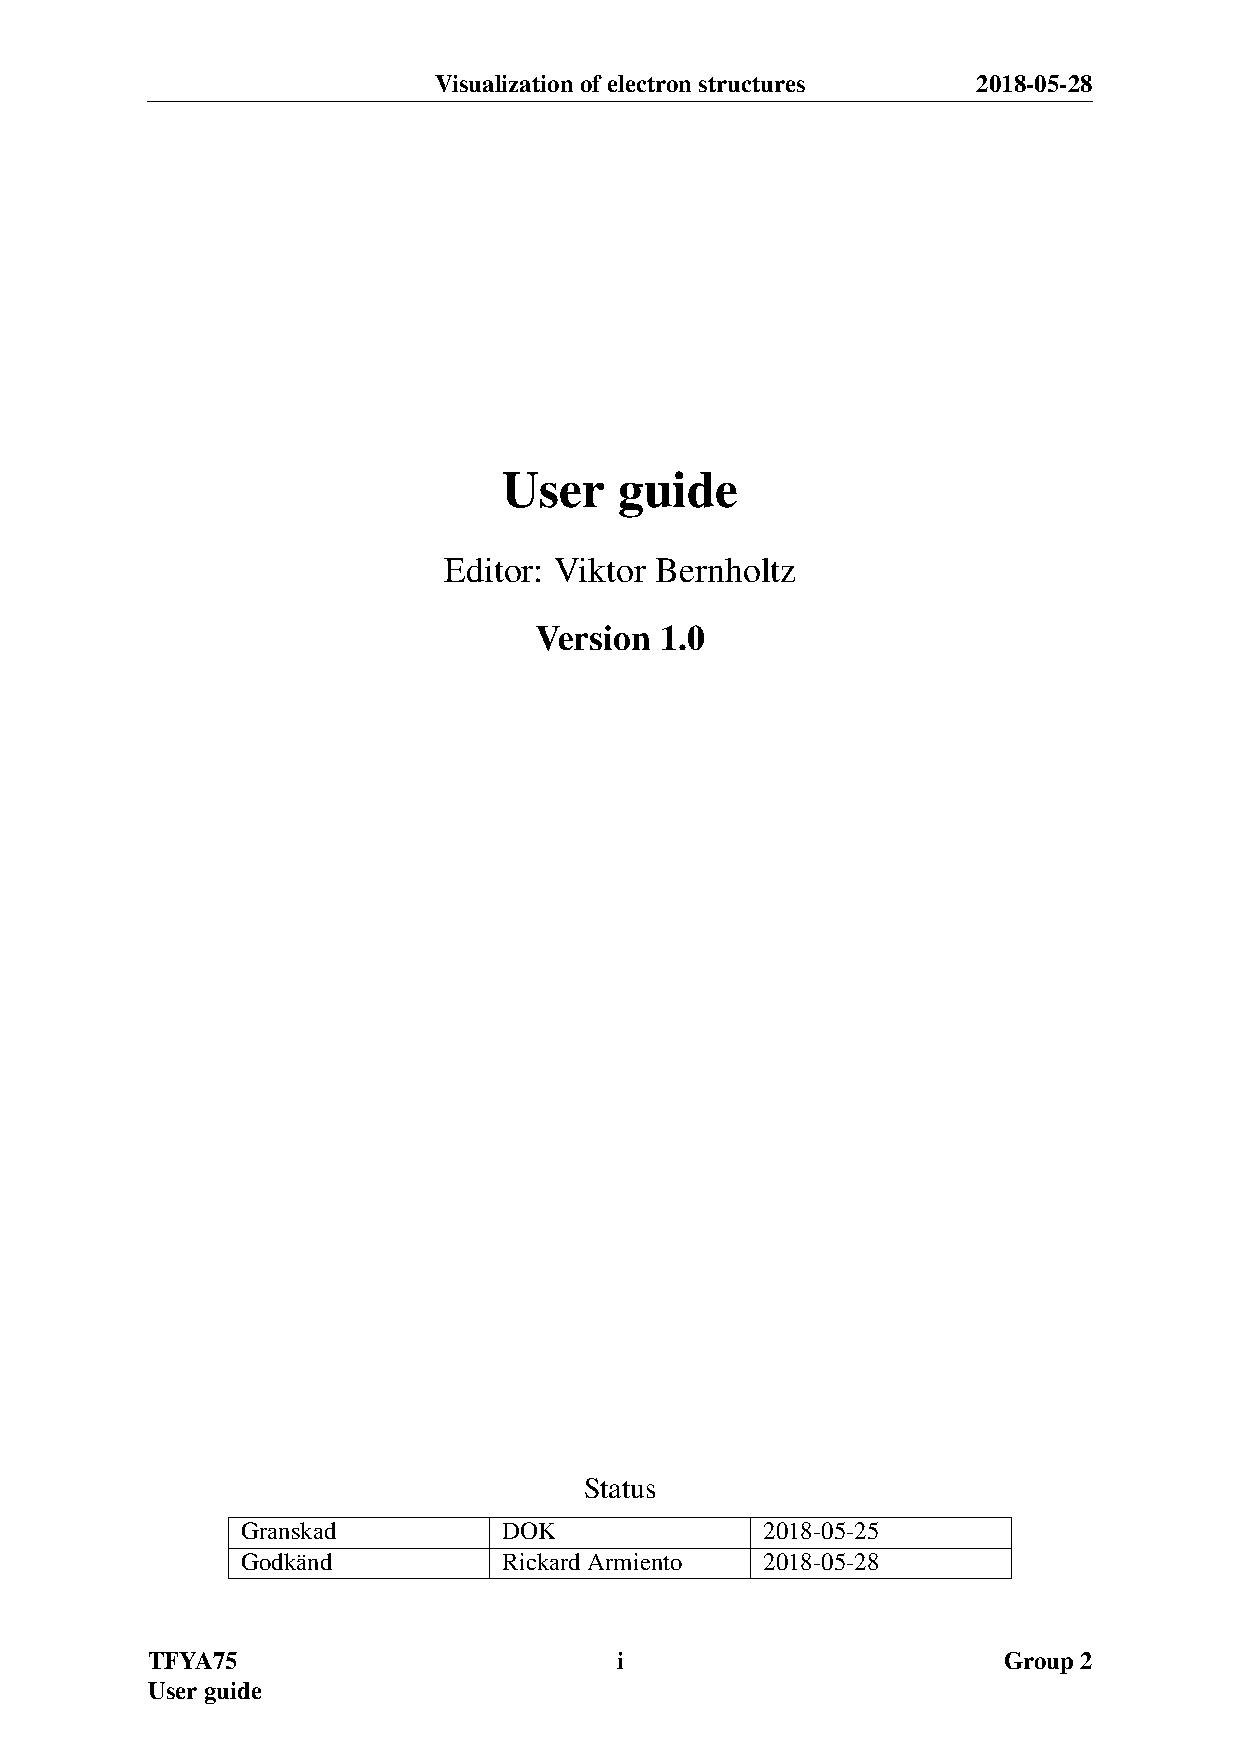
\includepdf[pages={1},pagecommand=\section{Användarmanual}\label{appendix:anvandarmanual}\thispagestyle{empty}]{user_guide.pdf} \includepdf[pages={2-}]{user_guide.pdf}
	
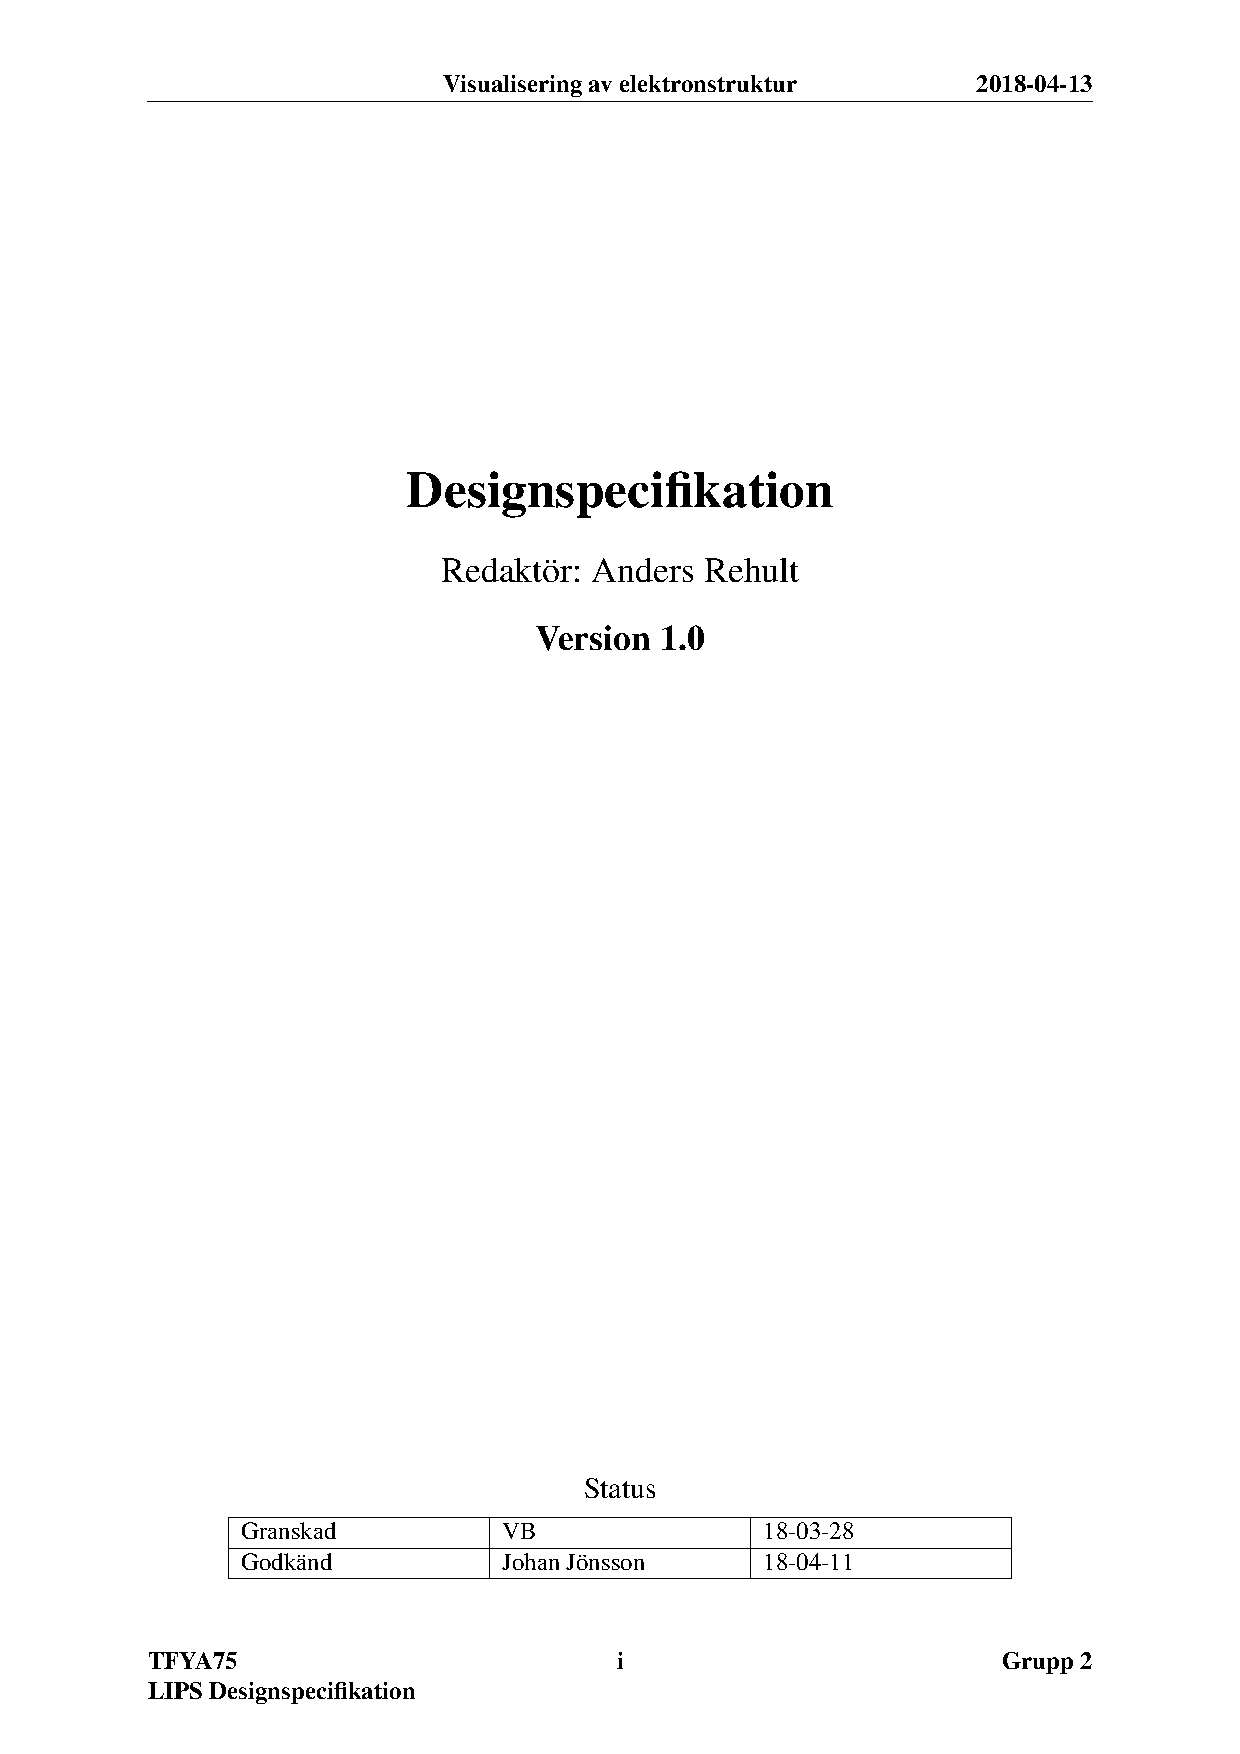
\includepdf[pages={1},pagecommand=\section{Designspecifikation}\label{appendix:designspecifikation}\thispagestyle{empty}]{designspecifikation_10.pdf} \includepdf[pages={2-}]{designspecifikation_10.pdf}
	
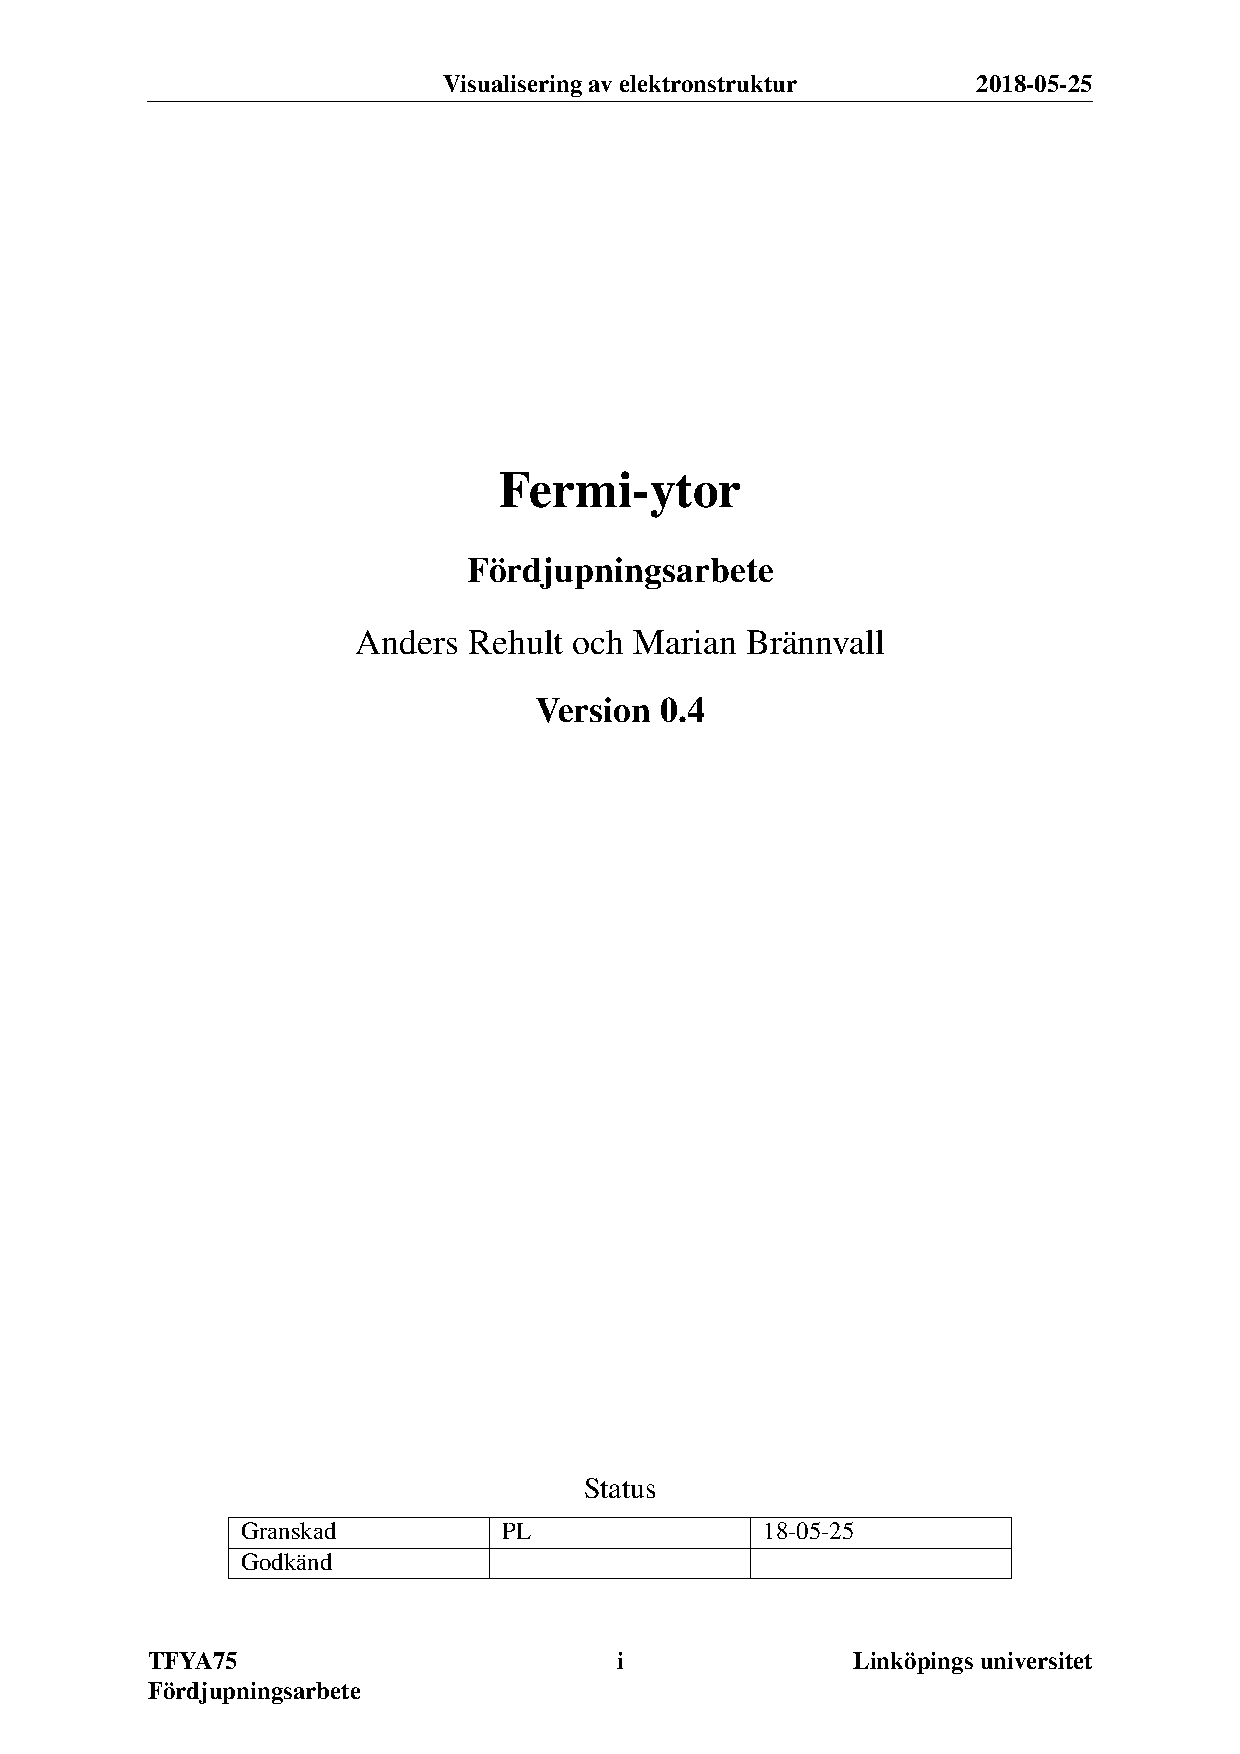
\includepdf[pages={1},pagecommand=\section{Fördjupningsarbete - Fermi-ytor }\label{appendix:fermi-ytor}\thispagestyle{empty}]{fordjupningsarbete-fermi-ytor.pdf}
\includepdf[pages={2-}]{fordjupningsarbete-fermi-ytor.pdf}

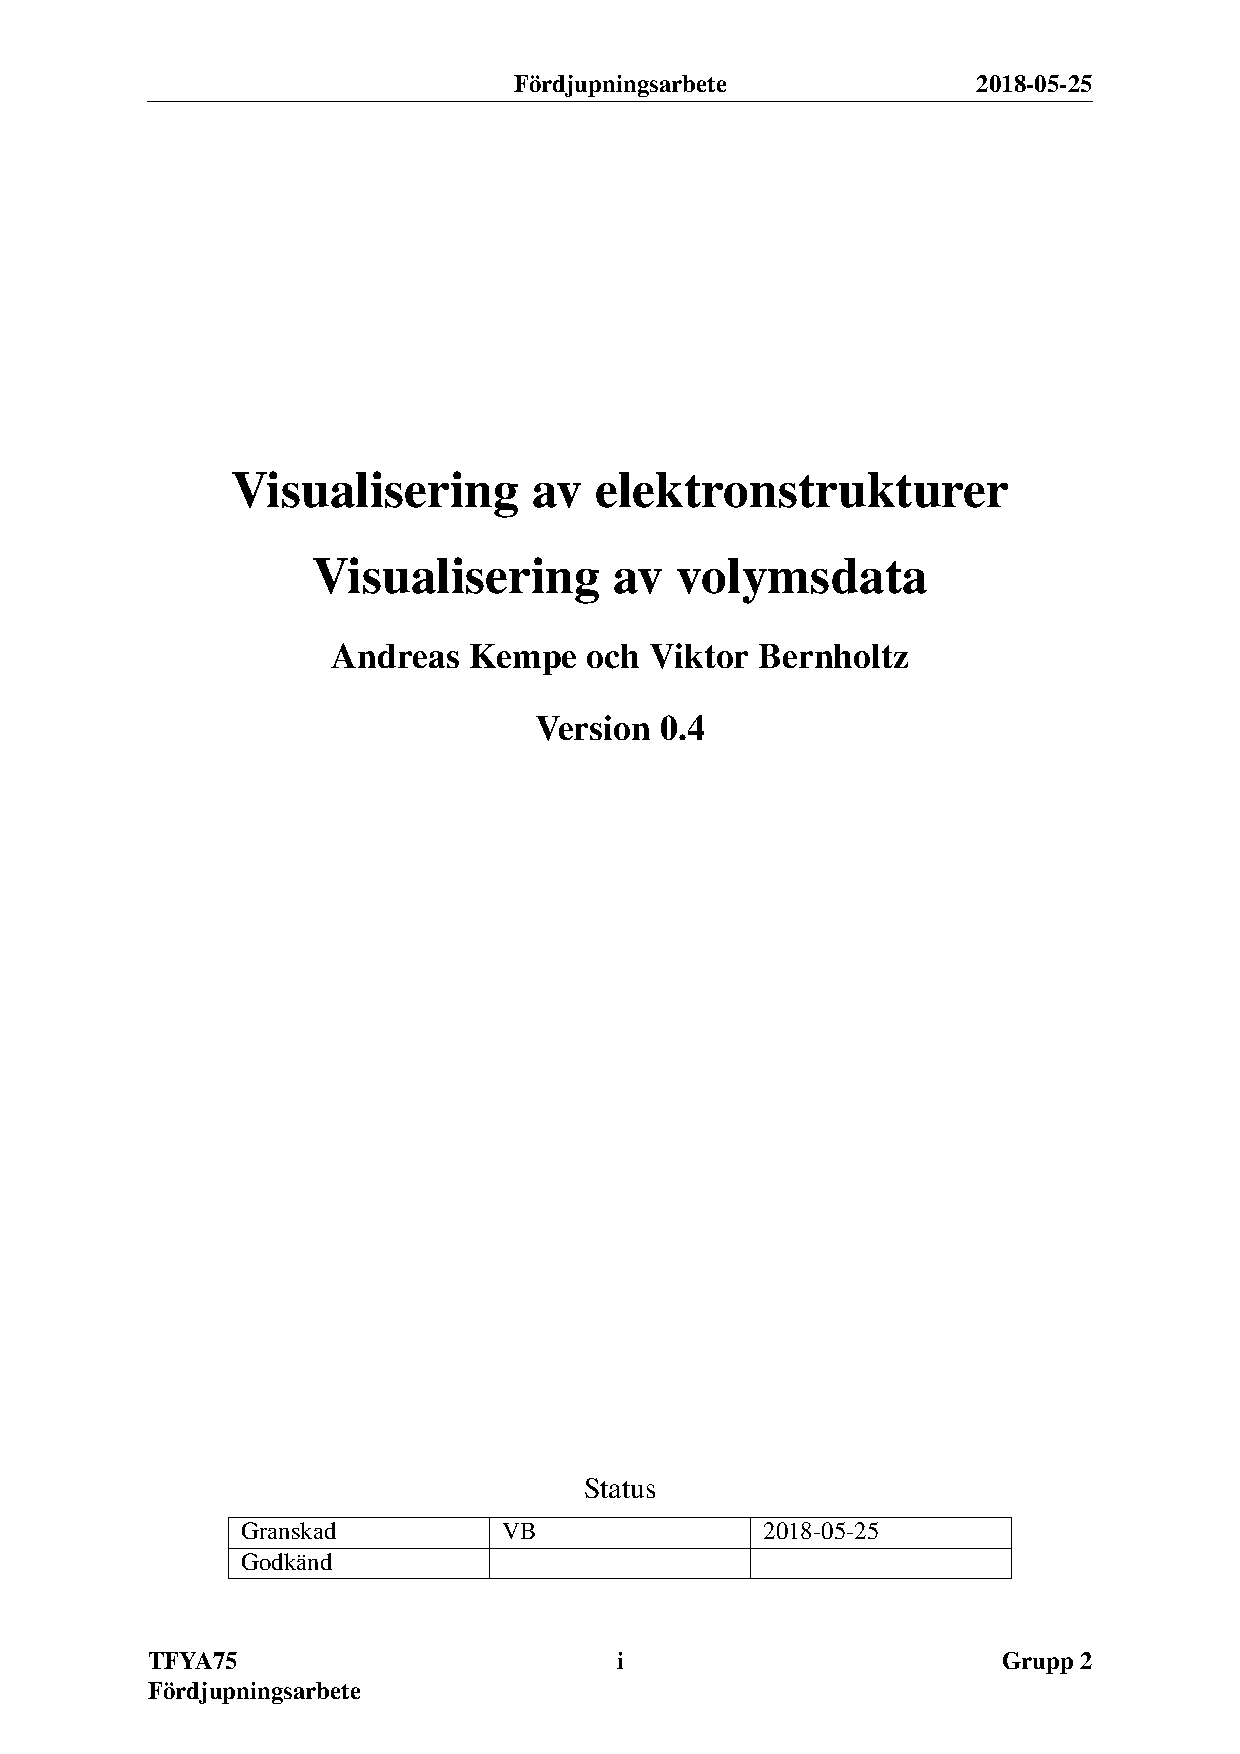
\includepdf[pages={1},pagecommand=\section{Fördjupningsarbete - Visualisering av volysmdata}\label{appendix:visualisering}\thispagestyle{empty}]{Visualisering-av-volymsdata.pdf}
\includepdf[pages={2-}]{Visualisering-av-volymsdata.pdf}
	
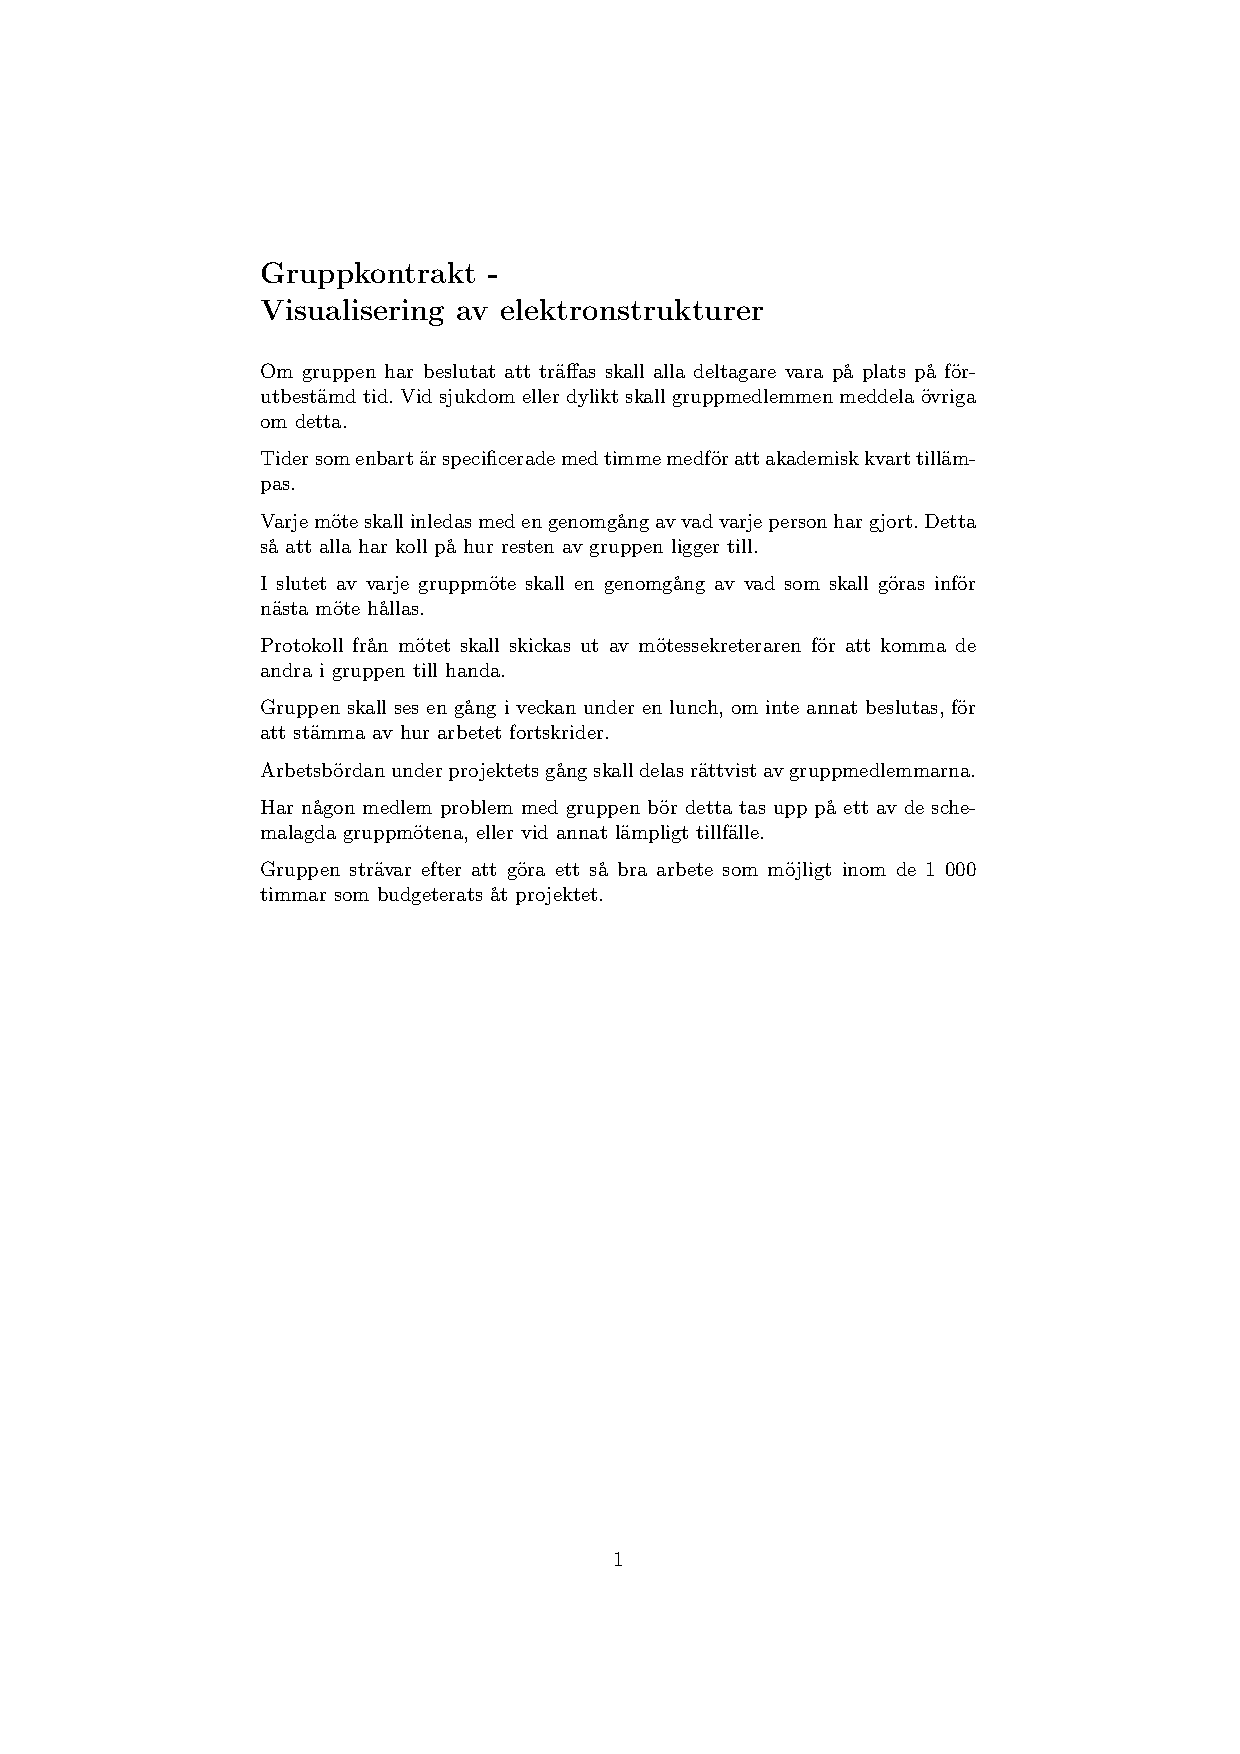
\includepdf[pages={1},pagecommand=\section{Gruppkontrakt}\label{appendix:Gruppkontrakt}\thispagestyle{empty}]{Gruppkontrakt.pdf}
	
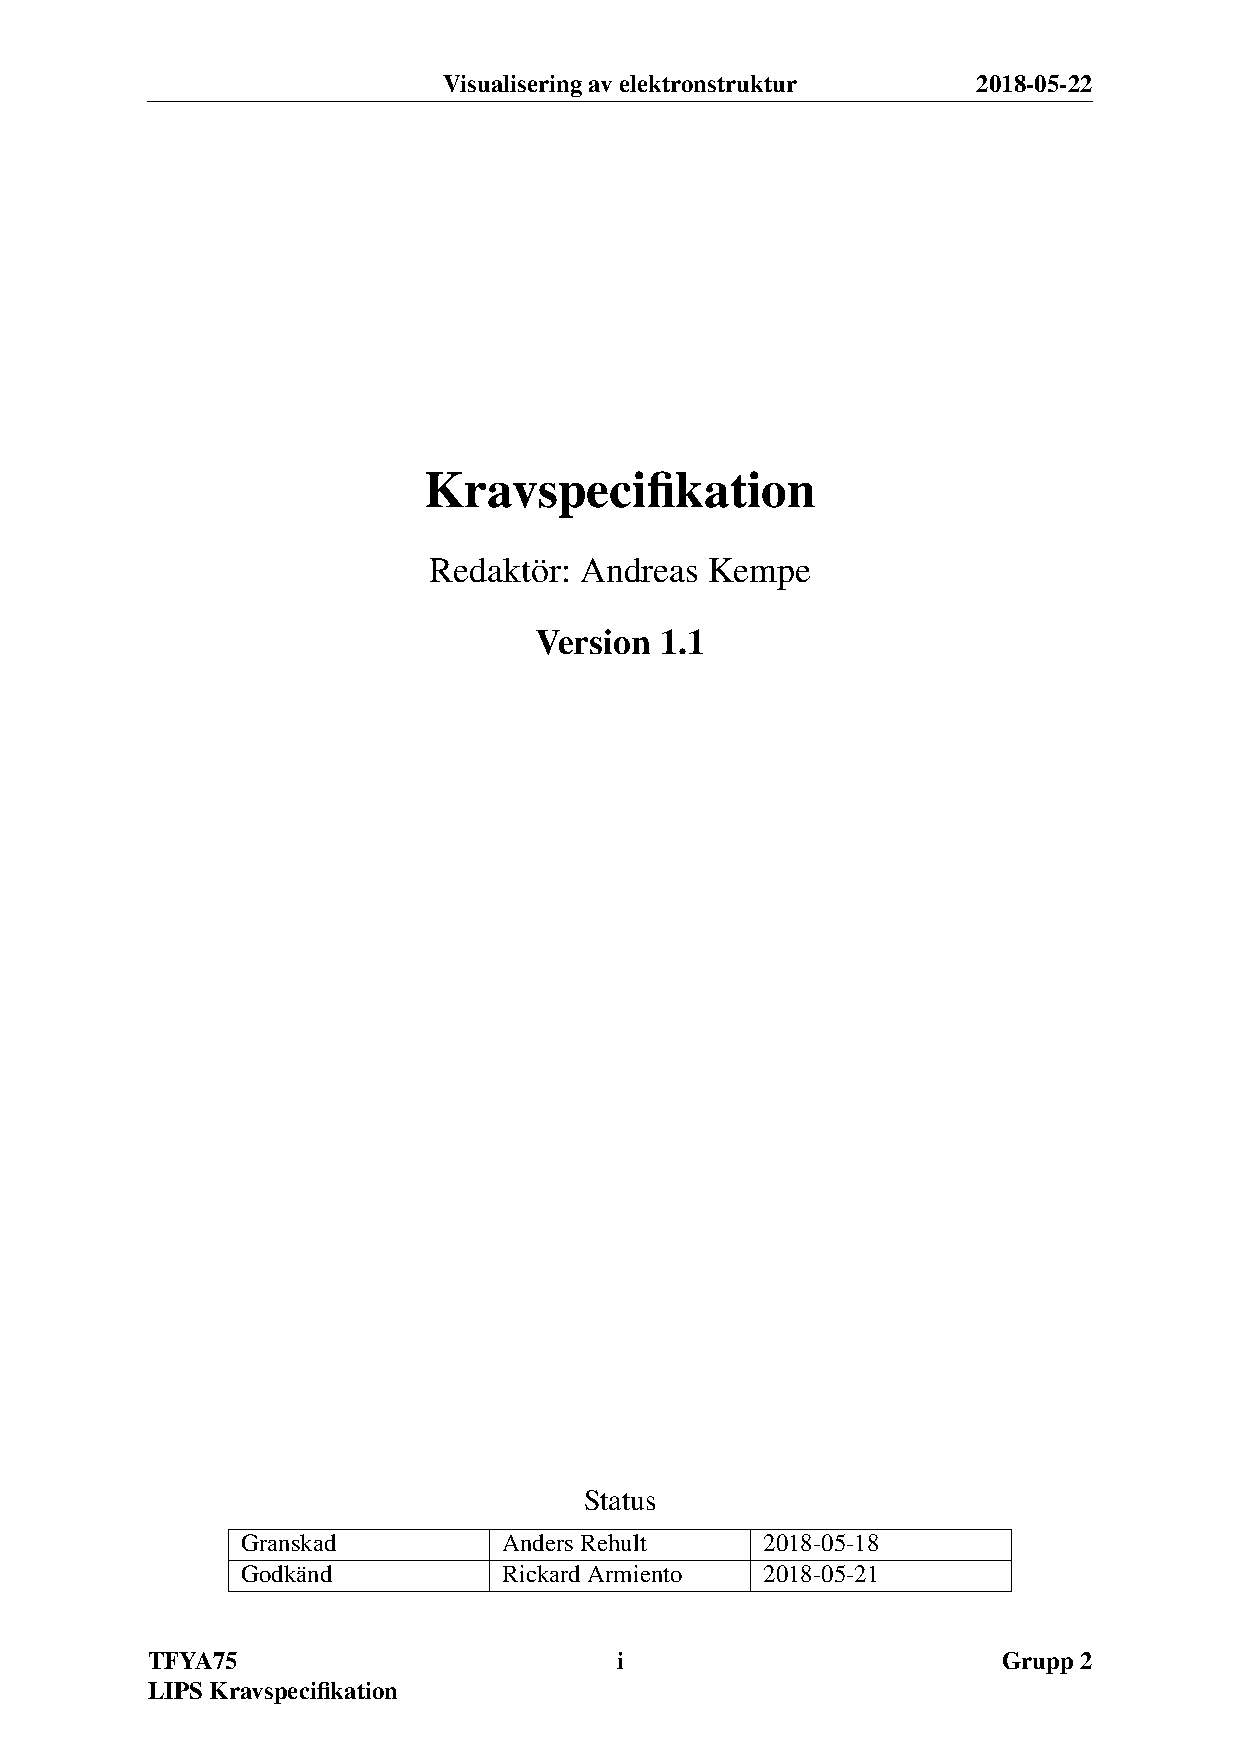
\includepdf[pages={1},pagecommand=\section{Kravspecifikation}\label{appendix:kravspecifikation}\thispagestyle{empty}]{Kravspecifikation.pdf}	\includepdf[pages={2-}]{Kravspecifikation.pdf}
	
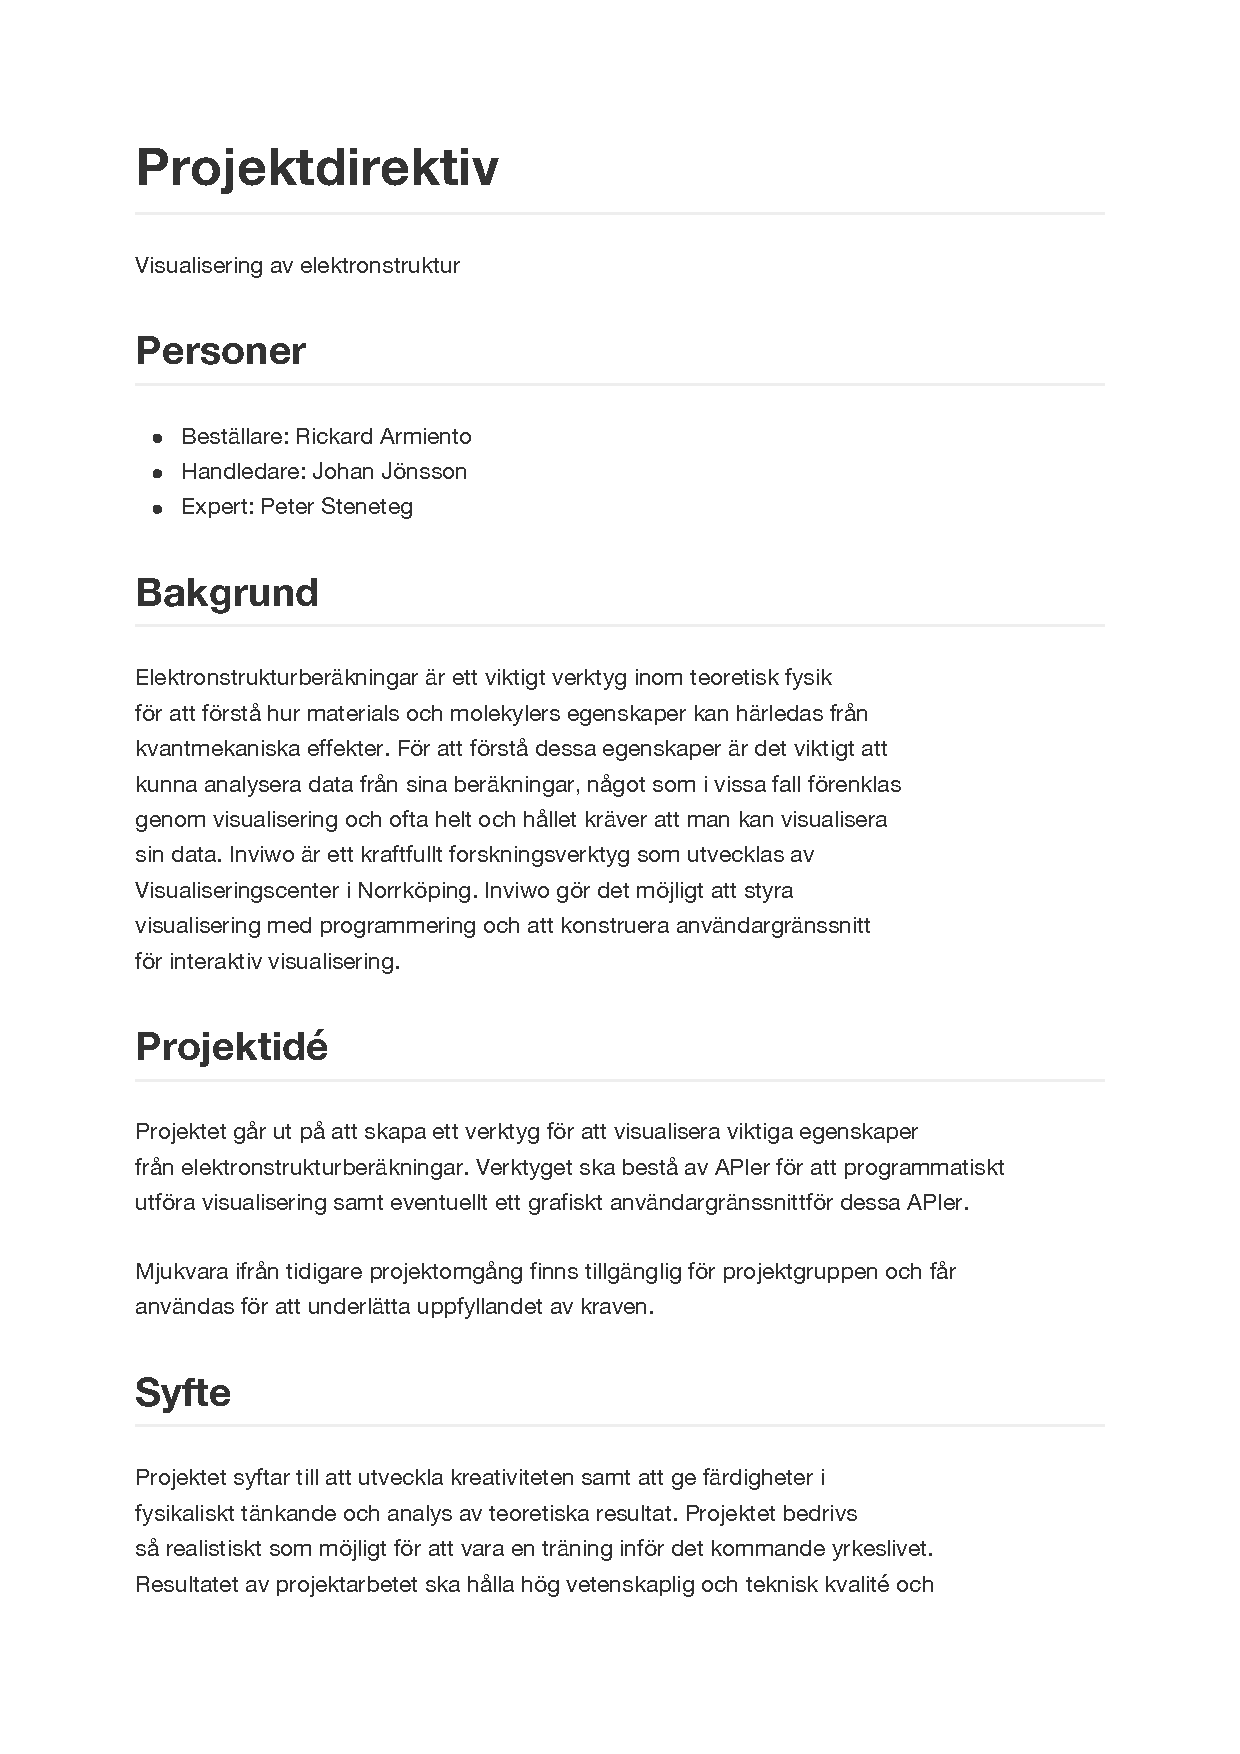
\includepdf[pages={1},pagecommand=\section{Projektdirektiv}\label{appendix:projektdirektiv}\thispagestyle{empty}]{projektdirektiv.pdf}
\includepdf[pages={2-}]{projektdirektiv.pdf}
	
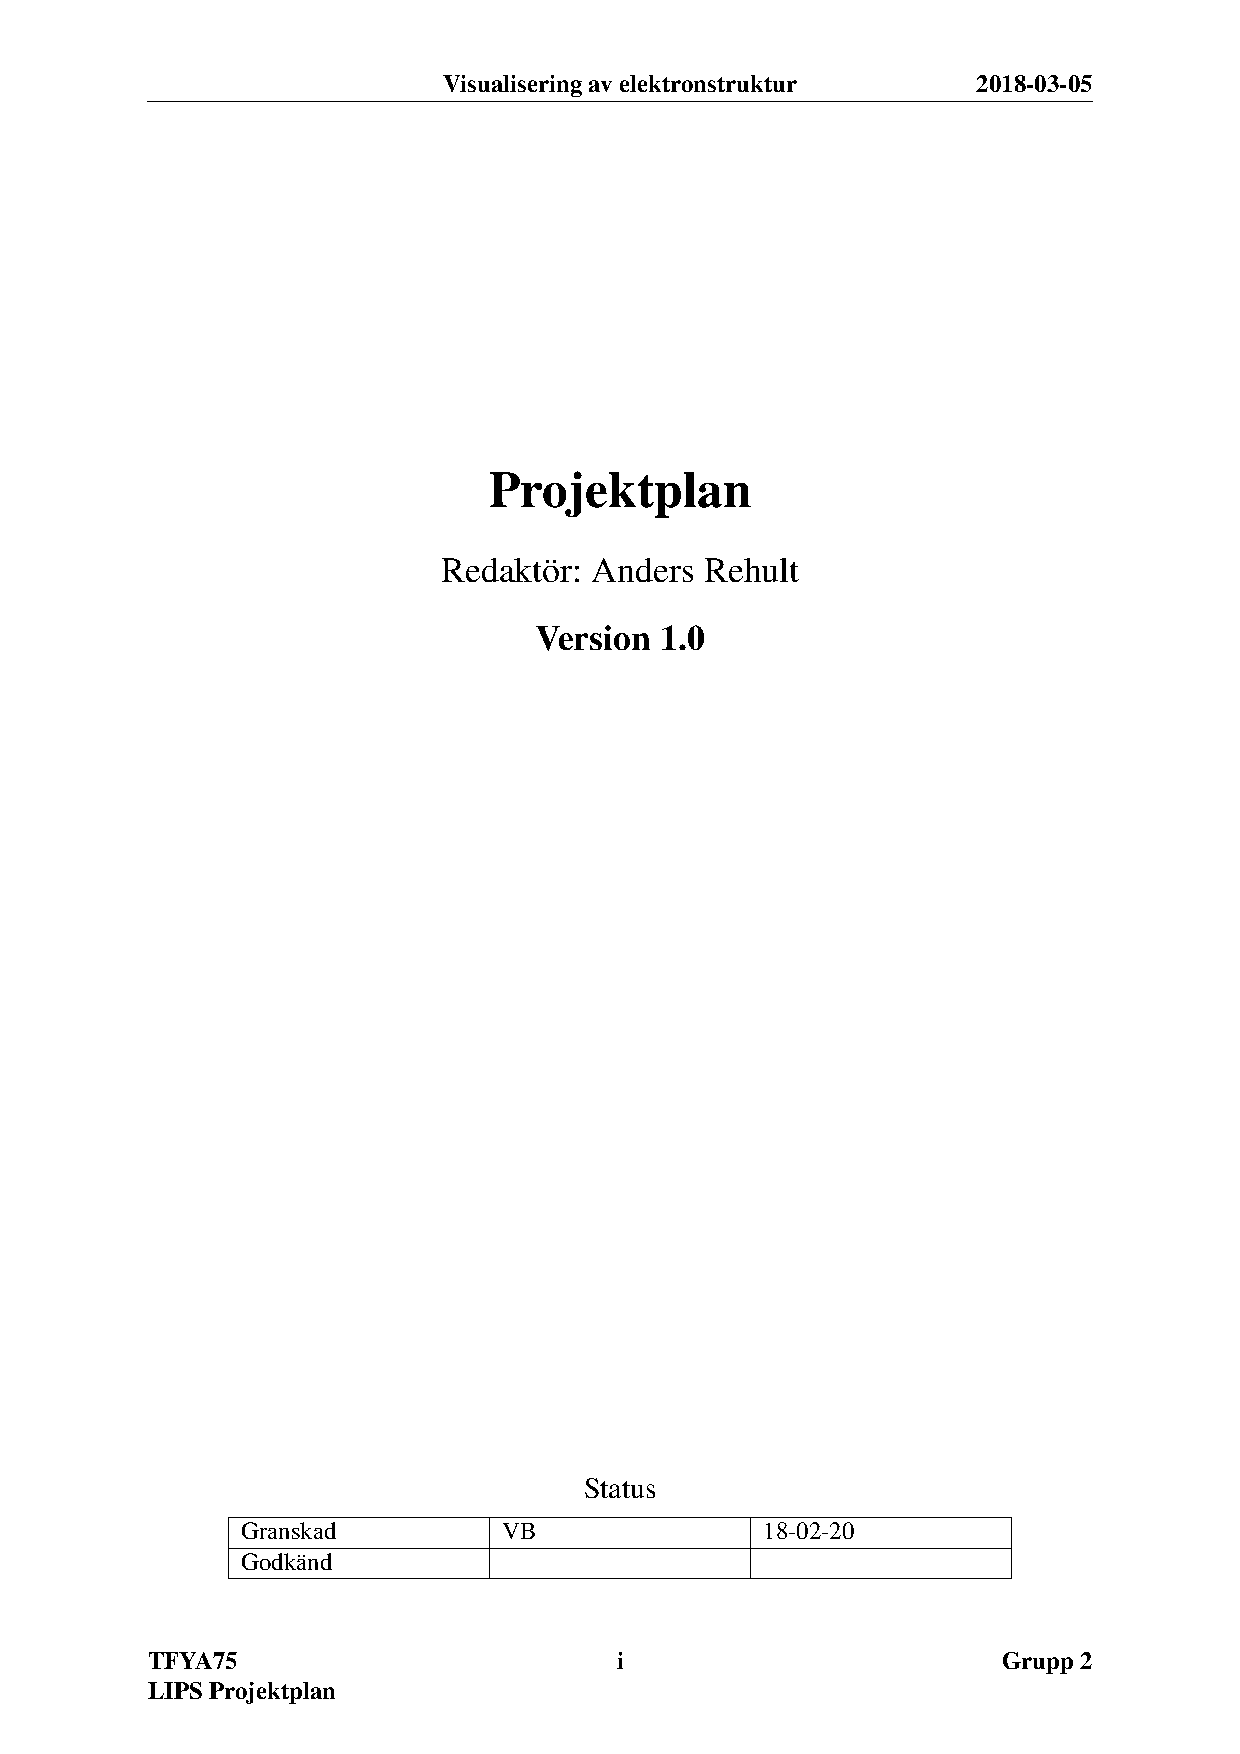
\includepdf[pages={1},pagecommand=\section{Projektplan}\label{appendix:projektplan}\thispagestyle{empty}]{projektplan.pdf}
\includepdf[pages={2-}]{projektplan.pdf}
	
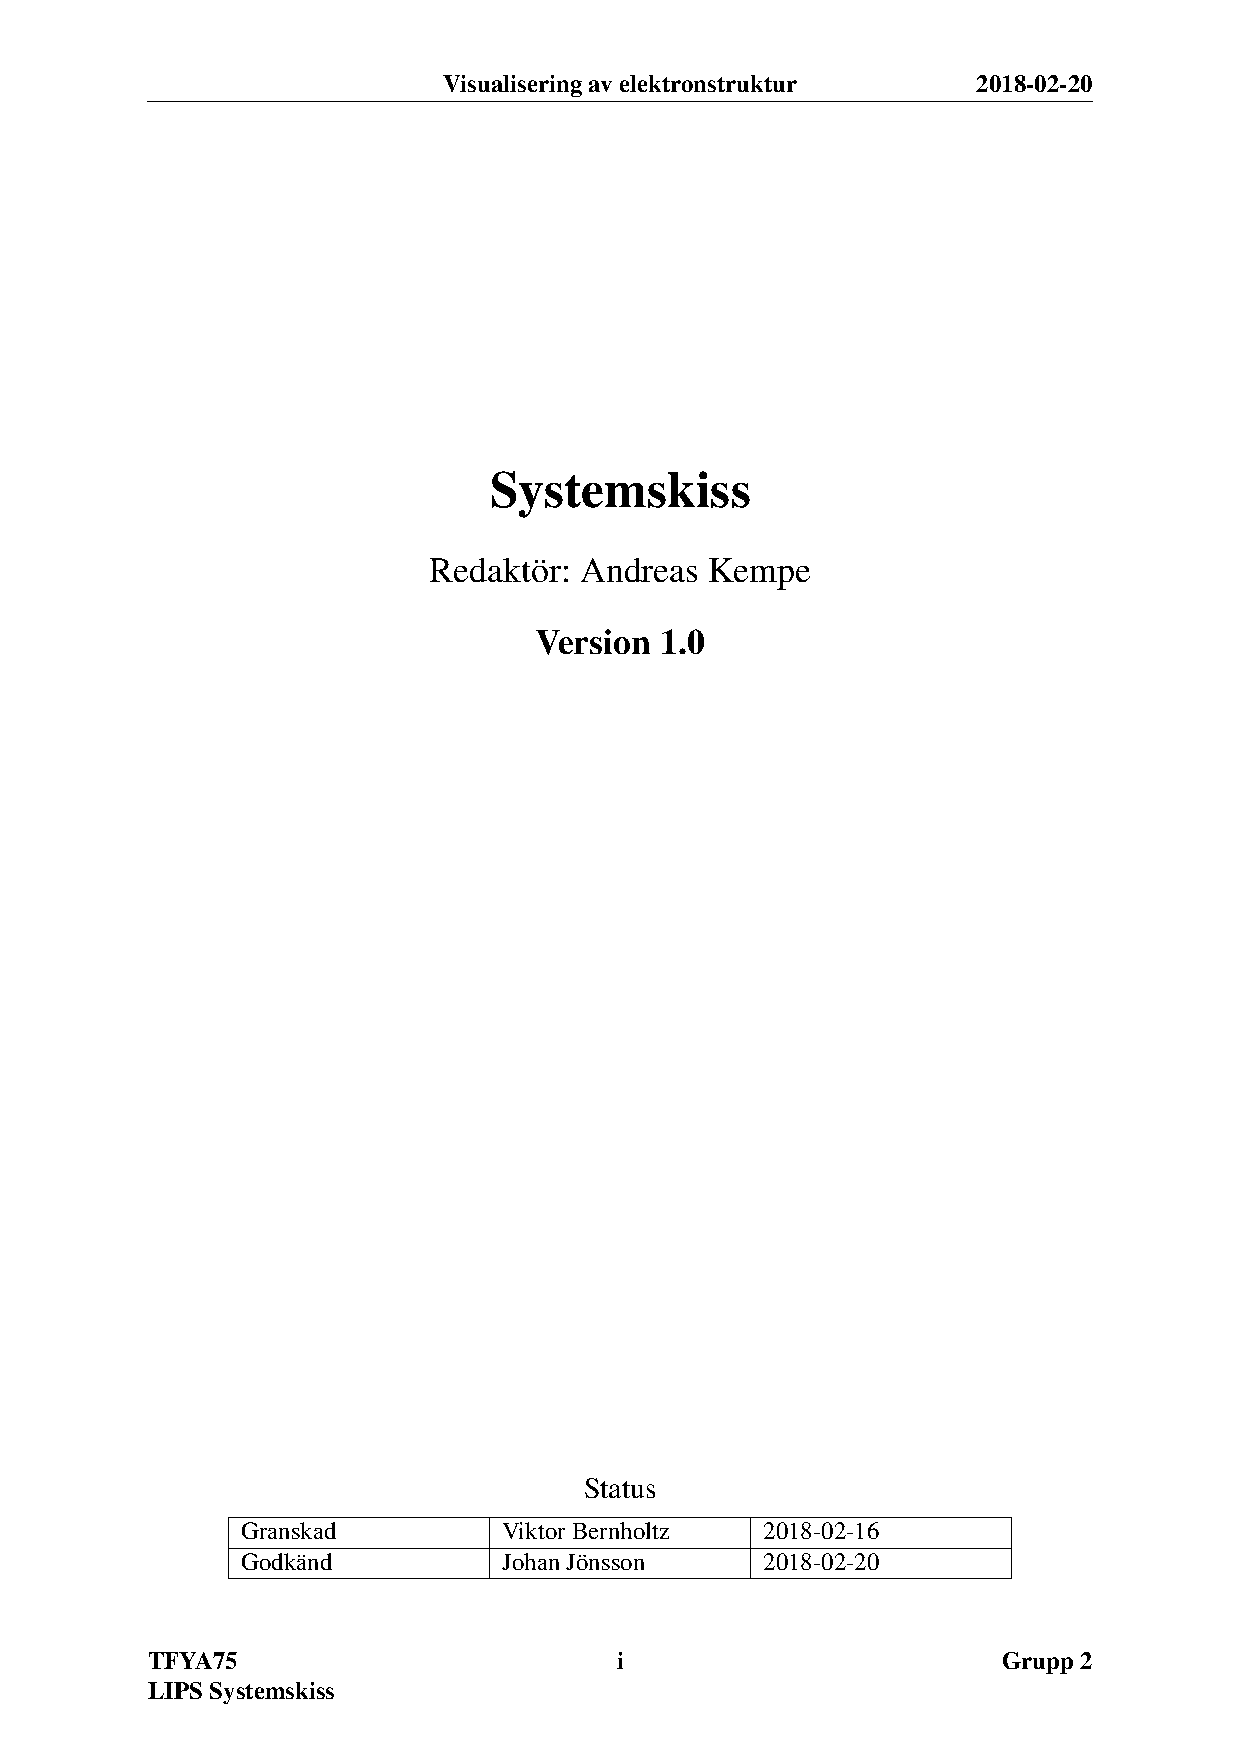
\includepdf[pages={1},pagecommand=\section{Systemskiss}\label{appendix:systemskiss}\thispagestyle{empty}]{Systemskiss.pdf}
\includepdf[pages={2-}]{Systemskiss.pdf}
	
	
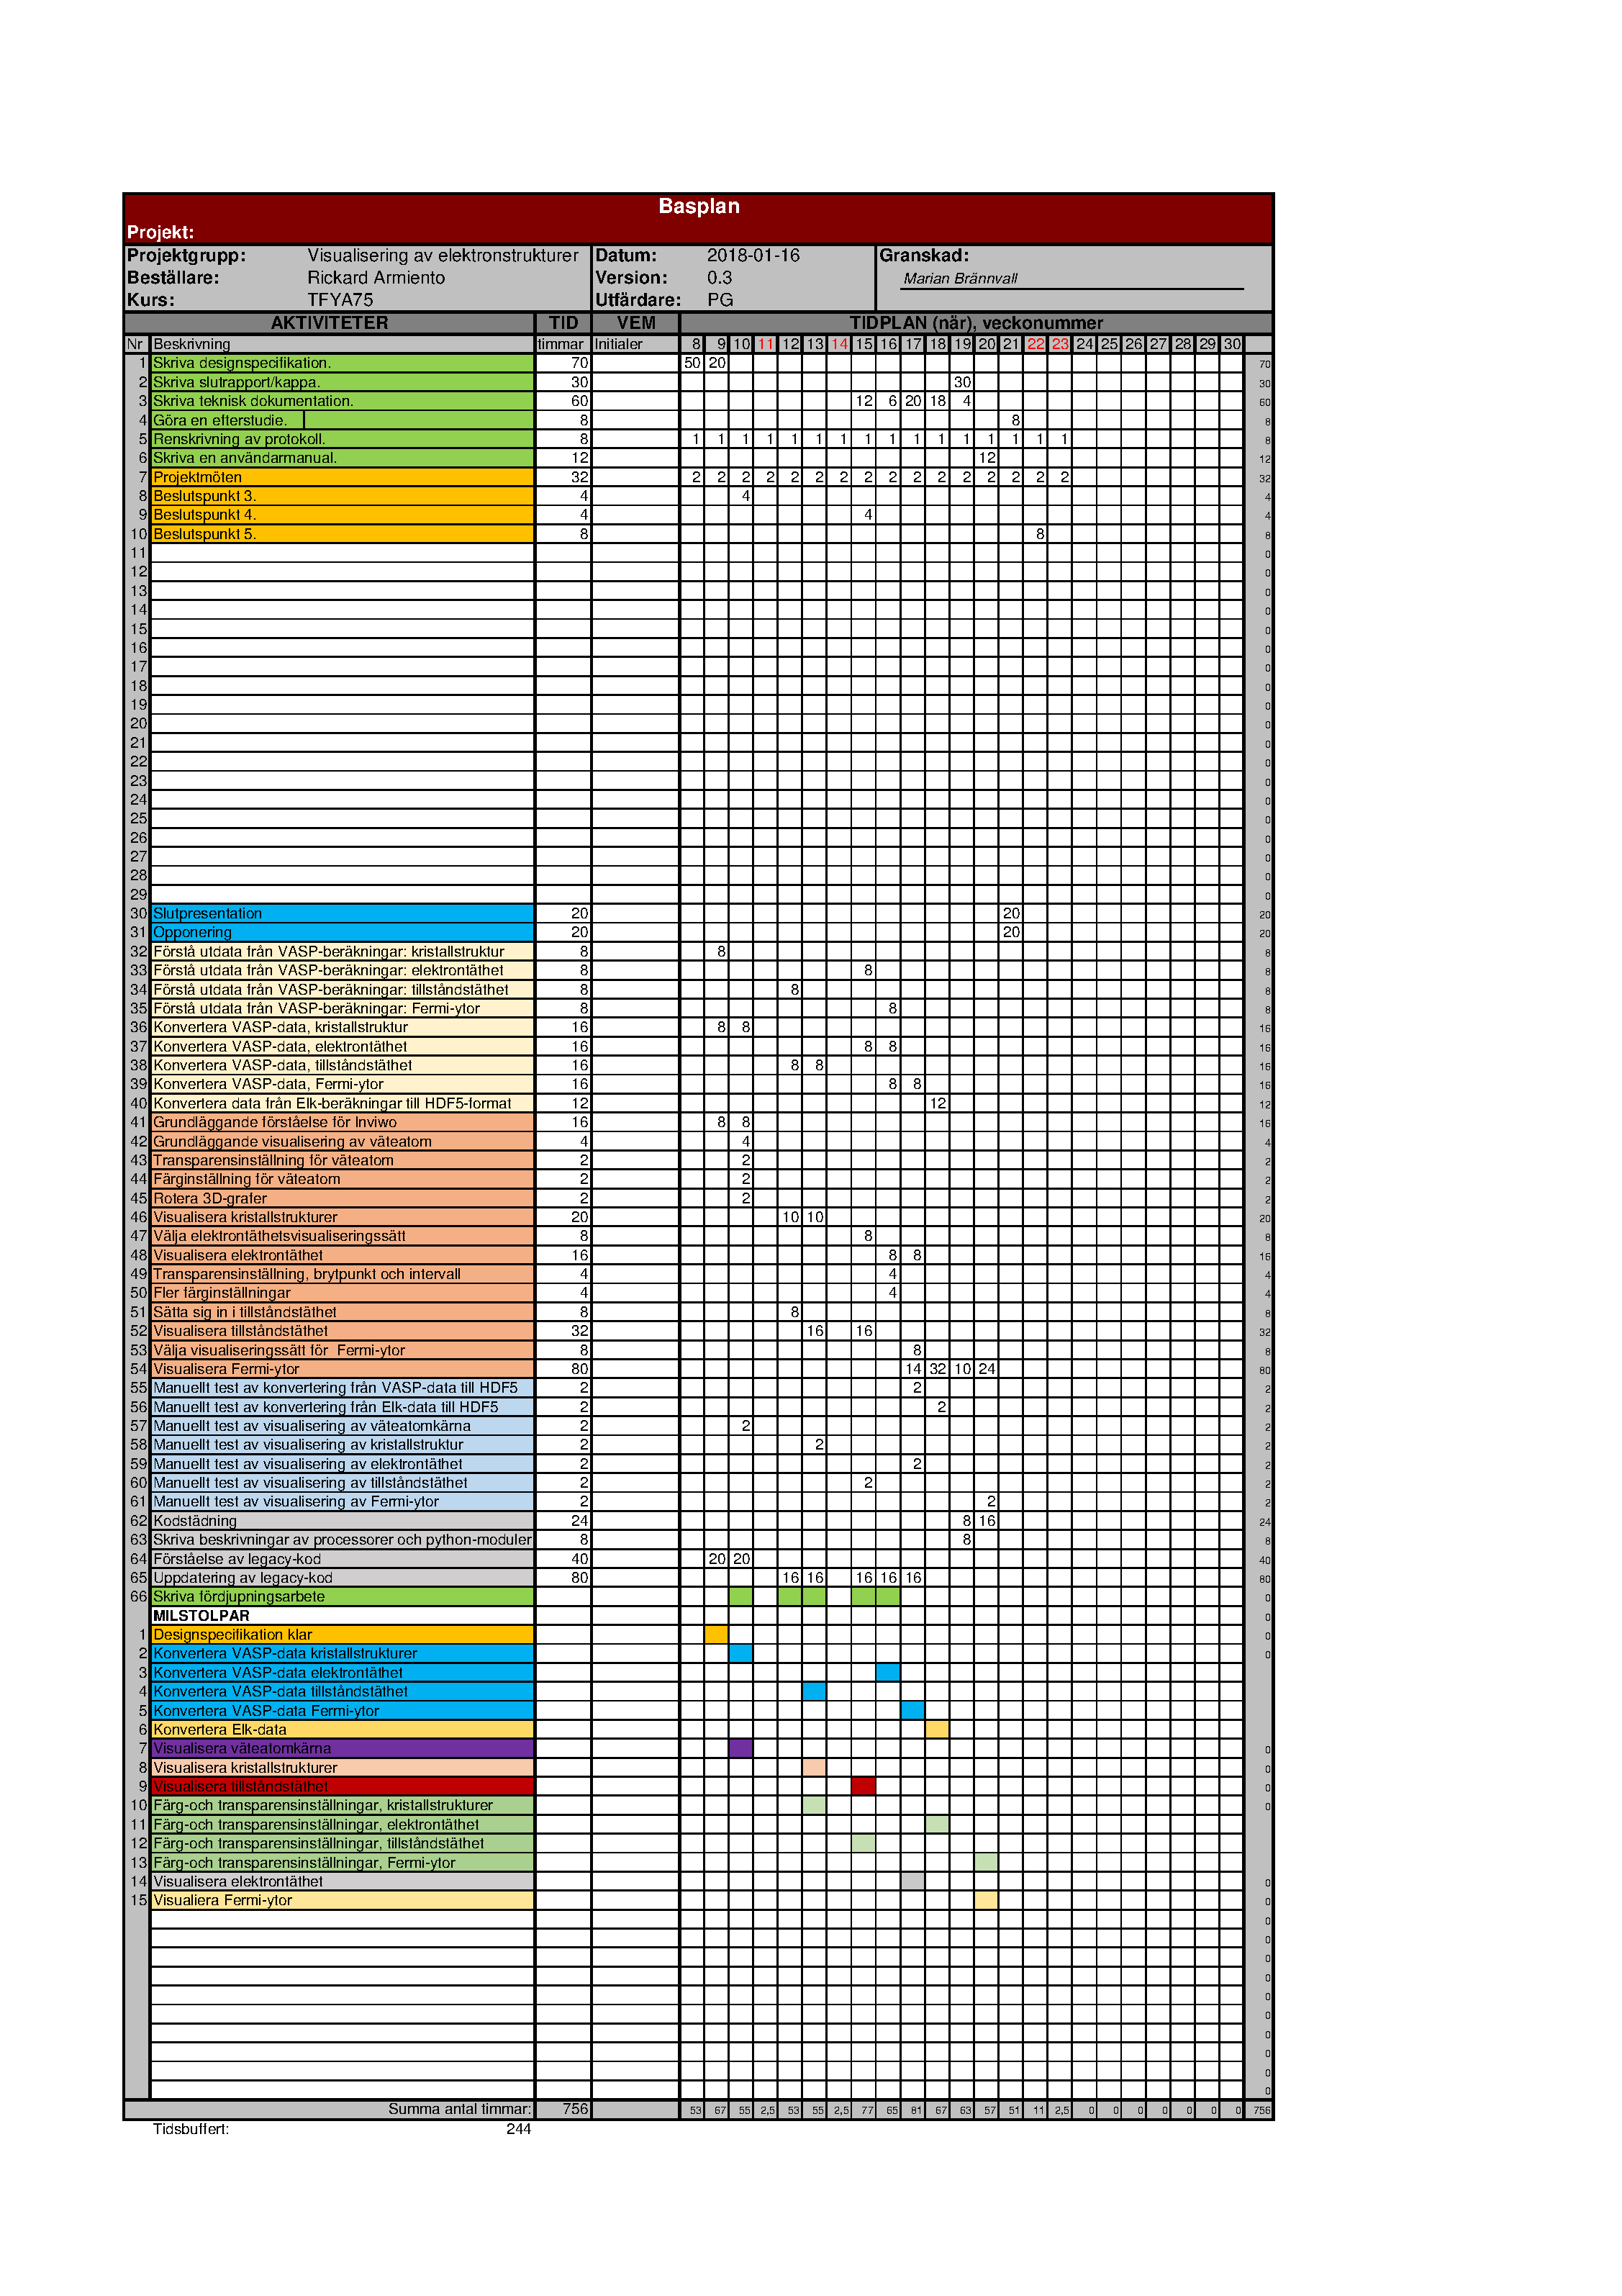
\includepdf[pages={1},pagecommand=\section{Tidplan}\label{appendix:tidplan}\thispagestyle{empty}]{tidplan.pdf}
	
	
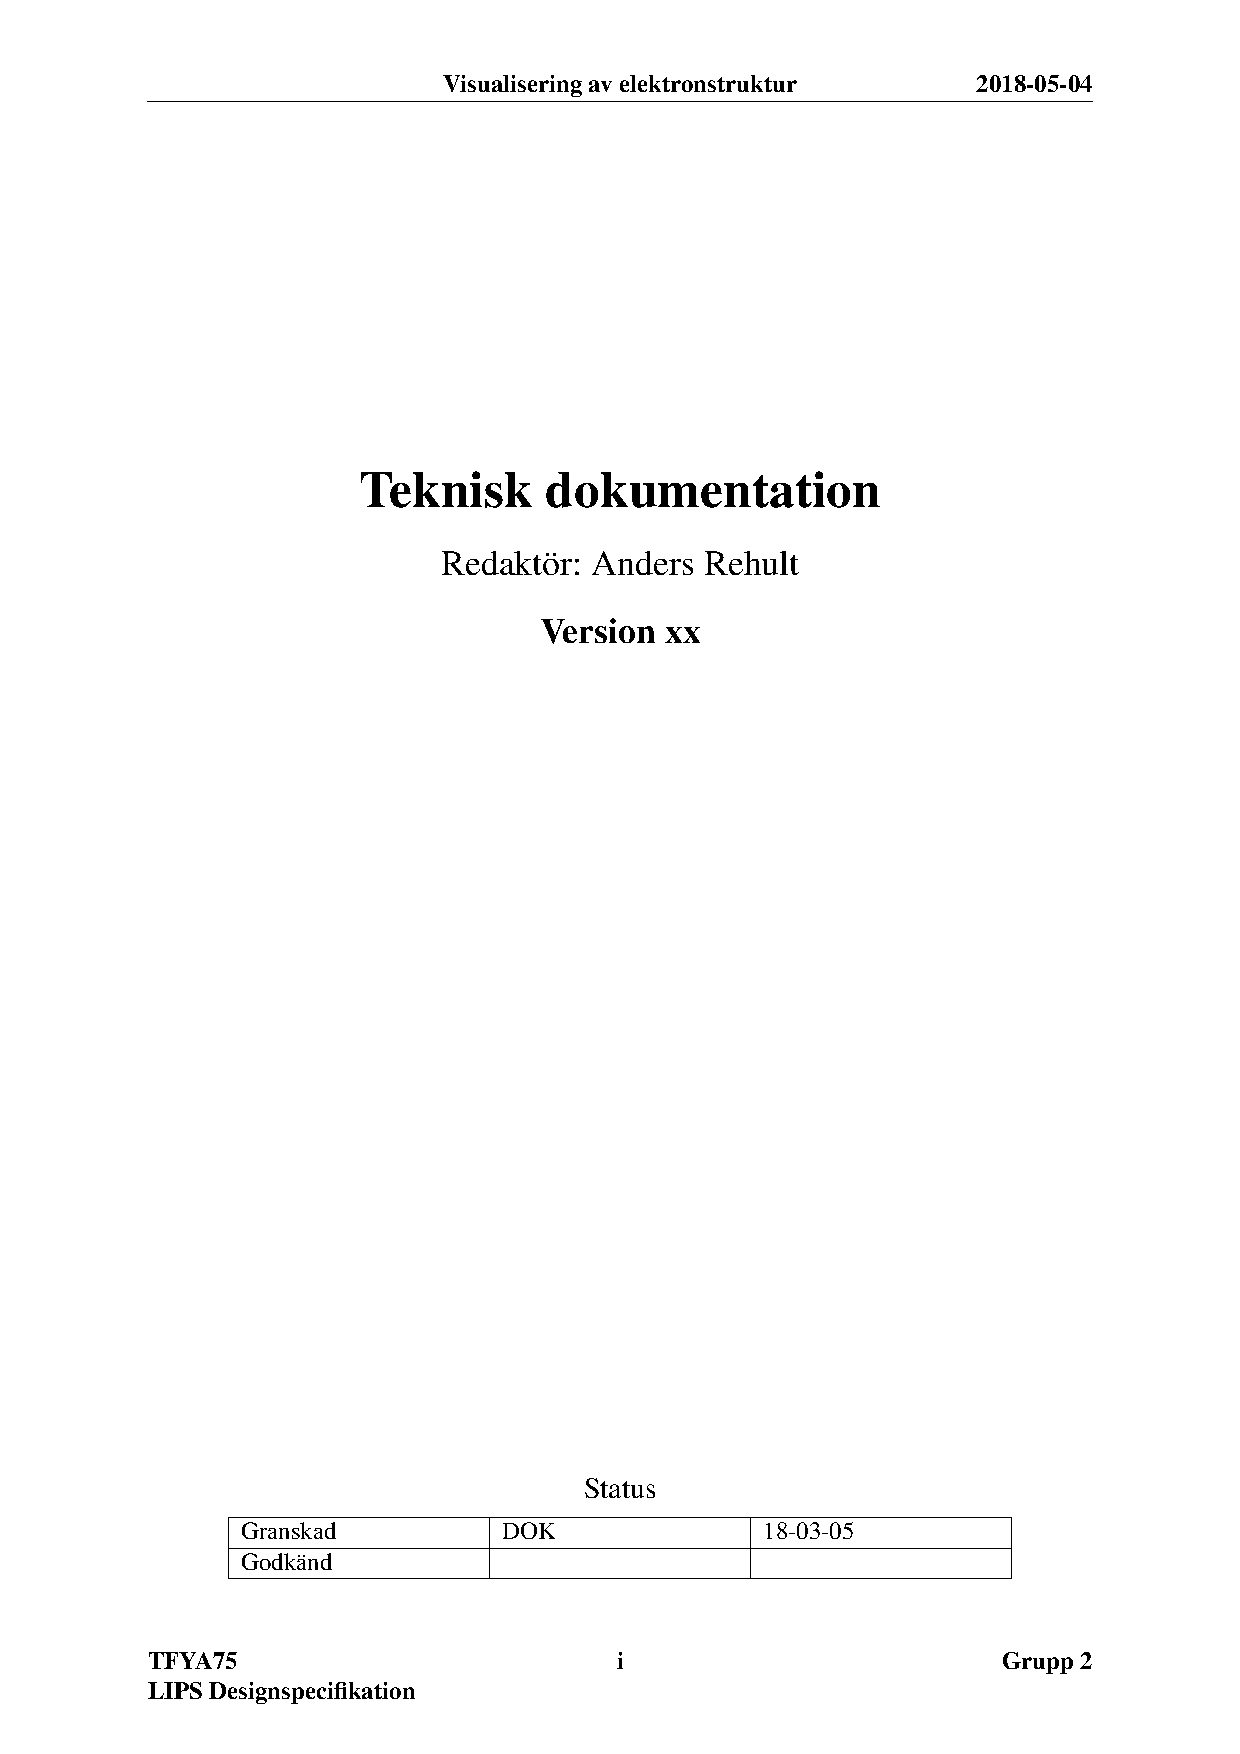
\includepdf[pages={1},pagecommand=\section{Teknisk dokumentation}\label{appendix:teknisk-dokumentation}\thispagestyle{empty}]{tekdok.pdf}
\includepdf[pages={2-}]{tekdok.pdf}

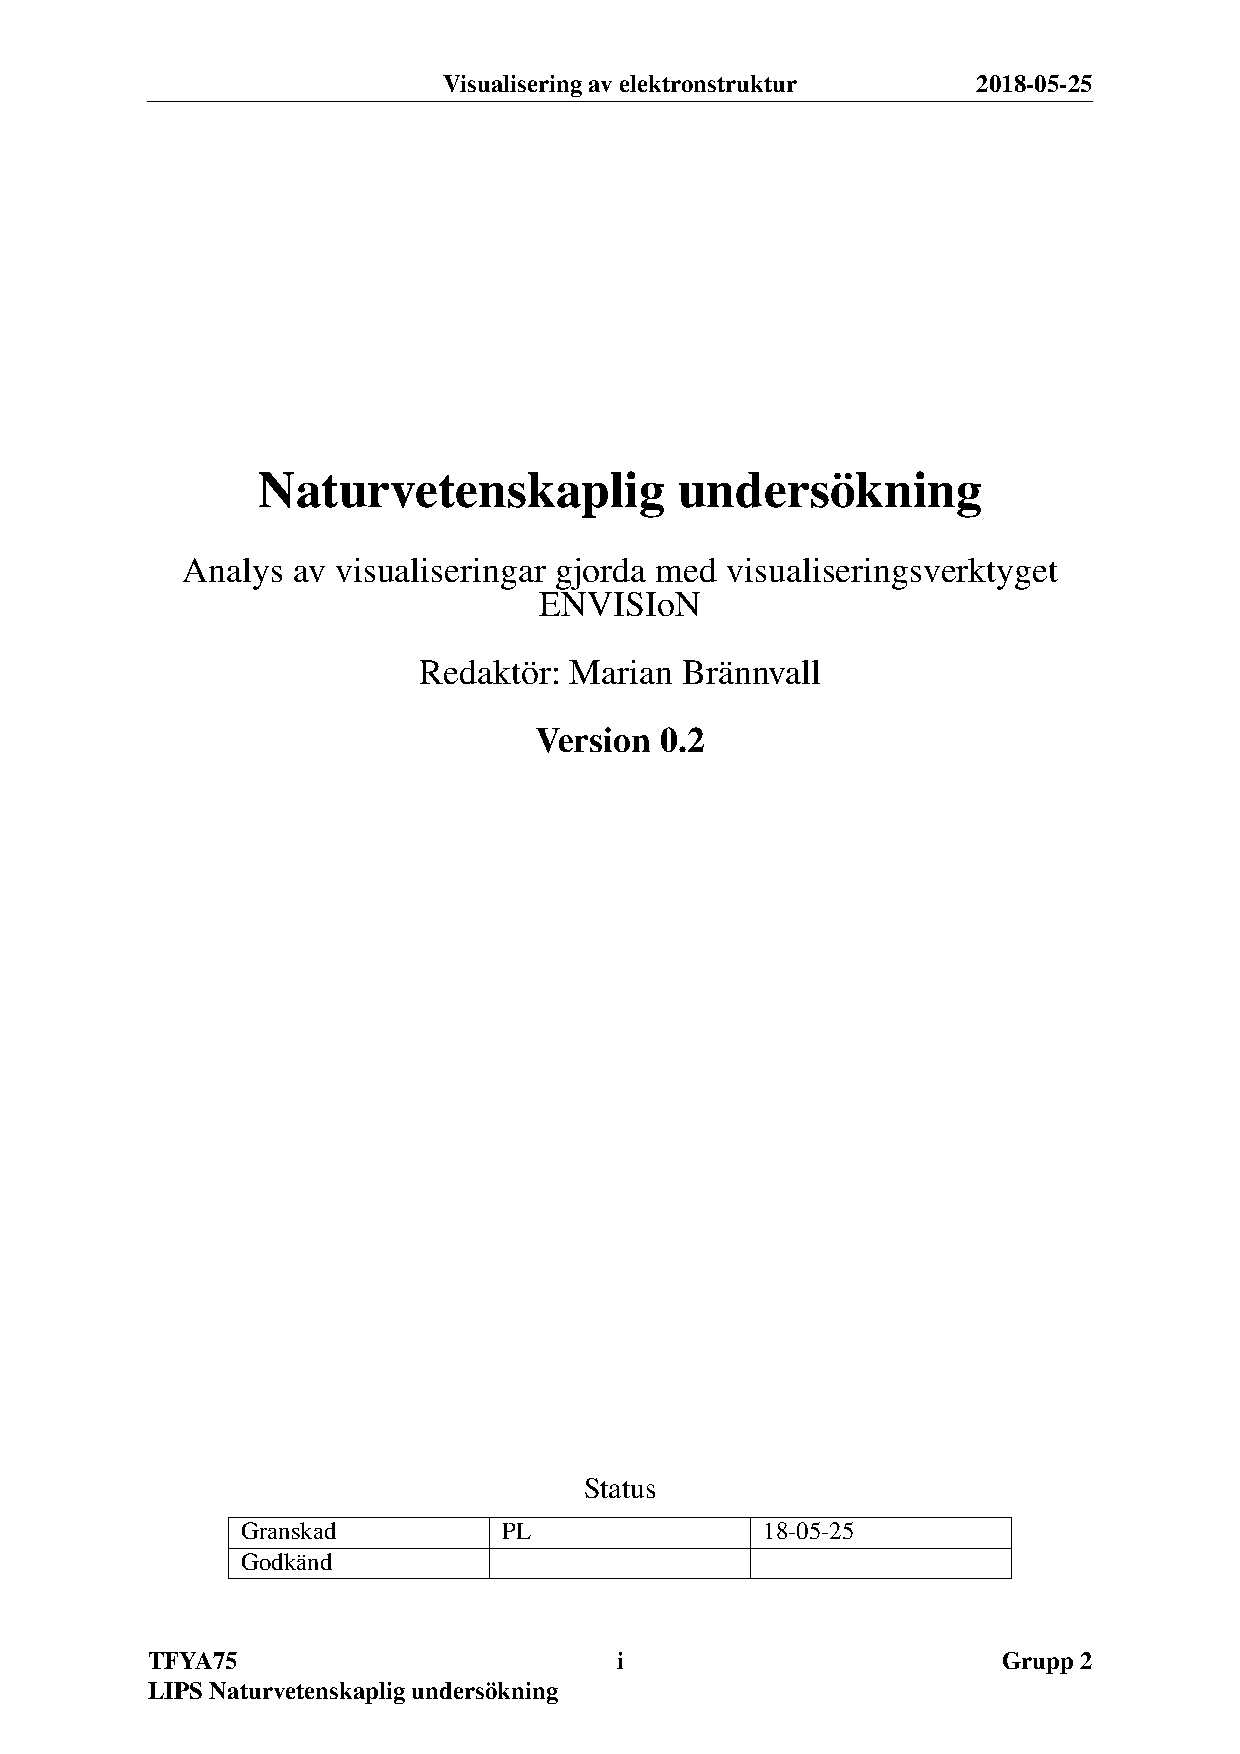
\includepdf[pages={1},pagecommand=\section{Naturvetenskaplig undersökning}\label{appendix:naturvetenskaplig}\thispagestyle{empty}]{naturvetenskaplig-undersokning.pdf} \includepdf[pages={2-}]{naturvetenskaplig-undersokning.pdf}

\end{appendices}

\end{document} 
